%%%%%%%%%%%%%%%%%%%%%%%%%%%%%%%%%%%%%%%%%%%%%%%%%%%%%%%%%%%%%%%%%%%%%%%%%%%%%%%%%%%
%%Anna University sample latex thesis format for UG thesis
%--------------------------------
%%This is the main file that includes the front matter and other chapter links. 
%%Chapters are placed within the folder named 1, 2,...  
%%To compile, run the command `pdflatex authesis.tex' in the terminal. 
%%Some packages may not be needed. Comment the ones, that are not needed. 
%%Images can be saved in the format of *.png. 
%%------------------------------------------------------
%% Authors:
%%Originally used by Dr. Mary Anita Rajam and then modified by Dr. Bama Srinivasan according to the latest Anna University regulations. %%Please report changes to bama@annauniv.edu, chorse@gmail.com %%
%%Acknowledgement: Thanks to Dr.Ranjani Parthasarathi, who relentlessly and patiently guided Bama Srinivasan.
%---------------------------------------------------------
%% Modification added:
%%new file apalikem is added, which gives a neat reference list with 1, 2...
%%aureportm has appendix starting with Arabic numbers
%% Disclaimer: Check with the latest Anna University regulations before working with this format.
%% Changes as on July 2016 
%% 1. Changed the appendix back to alpha mode in aureport.cls
%% 2. Table of contents - reduced the top margin and spacing
%% 3. Added the counter depth for sections to 4 in aureport.cls
%% 4. Deleted chapter number, title and page number in TOC
%% 5. Reduced the top space in chapter titles from 6.5 cms to 5.5 cms in aureport.cls
%% 6. Changes in references use the package natbib and style unsrt. Include a .bib file for the bibliography
%$$$$$$$$$$$$$$$$$$$$$$$$$$$$$$$$$$$$$$$$$$$$$$$$$$$$$$$$$$$$$$$$$$$$$$$$$$$$$$$$$$$$$$$$$$

\documentclass[13 pt,a4paper]{aureportm}
\usepackage{mathptm}\usepackage{etex}
\reserveinserts{28}
\renewcommand{\normalsize}{\fontsize{13 pt}{14.6 pt}\selectfont}
%\usepackage{aunatbib}
%\usepackage{apalikem}
\usepackage{natbib}
\usepackage{ragged2e}
\usepackage{bussproofs} % for deduction rules 
\usepackage{auphd}
\usepackage{array}
\usepackage{tabularx}
%\usepackage[none]{hyphenat}
\usepackage[chapter]{algorithm}
\usepackage{algpseudocode}
\usepackage{multirow}
\usepackage{multicol}
\usepackage{float}
\usepackage{booktabs}
\usepackage{amsmath}
\usepackage{amssymb}
\usepackage{amsthm}
\usepackage{latexsym}
\usepackage{verbatim}
\usepackage{ifthen}
\usepackage{graphicx}
\usepackage{hyperref}
\usepackage{epsfig}
\usepackage{pslatex}
\usepackage{setspace}
\usepackage{titlesec}
\usepackage[subfigure]{tocloft}
\usepackage{subfigure}
\usepackage{longtable}
\usepackage{enumerate}
\usepackage{lscape}
\usepackage{tikz}
\usepackage{pgfplots}

\usepackage[english]{babel}
\usepackage{fontspec}

\babelprovide[import]{tamil}
\babelfont[tamil]{rm}{Noto Sans Tamil}

\usepackage[format=hang,labelfont=bf,textfont=bf]{caption}
\PassOptionsToPackage{linktocpage}{hyperref}
\tocloftpagestyle{myheadings}
\newcommand{\PreserveBackslash}[1]{\let\temp=\\#1\let\\=\temp}
\let\PBS=\PreserveBackslash

\usepackage{colortbl}
\usepackage{newlfont}


\newboolean{psoutput}
\setboolean{psoutput}{true}
\usepackage{pst-all}
\newcommand{\defname}[1]{\emph{#1}.}

\newtheorem{fact}{Fact}[chapter]

\floatstyle{ruled}
\newfloat{algorithm}{htp}{loa}
\floatname{algorithm}{Algorithm}


\titleformat{\section}[hang]{\bfseries}{\makebox[20mm][l]{\thesection}}{0pt}{}{}
\titleformat{\subsection}[hang]{\bfseries}{\makebox[20mm][l]{\thesubsection}}{0pt}{}{}



 \newcounter {definition}[chapter]
\renewcommand \thedefinition {\arabic{chapter}.\arabic{definition}}
\newenvironment{definition}
{ \refstepcounter{definition}
   {\noindent \bf Definition \arabic{chapter}.\arabic{definition}.}}
 {}
 \def\enddefinition{$\Box$}

 \newcounter {example}[chapter]
 \renewcommand \theexample
 {\arabic{chapter}.\arabic{example}}
 \newenvironment{example}
 { \refstepcounter{example}
   {\noindent \bf Example \arabic{chapter}.\arabic{example}.}}
 {}
 \def\endexample{$\Box$}

 \newcounter {proposition}[chapter]
 \renewcommand \theproposition {\arabic{chapter}.\arabic{proposition}}
 \newenvironment{proposition}
 {\refstepcounter{proposition}
   {\noindent \bf Proposition \arabic{chapter}.\arabic{proposition}. }}
 {}
 \def\endproposition{$\Box$}

\pagenumbering{roman}
\setcounter{page}{3}
%\setcounter{secnumdepth}{3}
\renewcommand{\baselinestretch}{1.5}
\newcommand{\row}{i}
\newcommand {\combined} {{C}}
\newcommand {\mtis} {}

\newboolean{showalter}
\setboolean{showalter}{true}
\newcommand{\alter}[1]{\ifthenelse{\boolean{showalter}}{ \{ #1 \} }{}}
\providecommand{\tabularnewline}{\\}
\newcommand{\bigsize}{\fontsize{15pt}{20pt}\selectfont}

\author{Author of the thesis}


\renewcommand{\cfttoctitlefont}{\bfseries\Large}
\renewcommand{\cftlottitlefont}{\bfseries\Large}
\renewcommand{\cftloftitlefont}{\bfseries\Large}


%\cftsetindents{chapter}{0mm}{10mm}
%\cftsetindents{section}{10mm}{10mm}
%\cftsetindents{subsection}{20mm}{10mm}
%\setlength{\cftbeforechapskip}{1.2\baselineskip}
%\setlength{\cftbeforesecskip}{.8\baselineskip}
%\setlength{\cftbeforesubsecskip}{.8\baselineskip}
%\setlength{\cftbeforefigskip}{.8\baselineskip}
%\setlength{\cftbeforetabskip}{.8\baselineskip}
%
\makeatletter
\renewcommand{\@dotsep}{10}
\makeatother
\renewcommand{\cftdot}{ }
\cftsetrmarg{1.2in} % changed by bama - earlier it was 1.5 inch. right margin is decreased to 1 inch.

\titleformat{\section}[hang]{\bfseries}{\makebox[20mm][l]{\thesection}}{0pt}{}{}
\titleformat{\subsection}[hang]{\bfseries}{{\thesubsection}}{0pt}{}{}
\titleformat{\subsubsection}[hang]{\normalsize\bfseries}{\makebox[20mm][l]{\thesubsubsection}}{0pt}{}{}
\titleformat{\paragraph}[hang]{\normalsize\bfseries}{\makebox[20mm][l]{\theparagraph}}{0pt}{}{}
\titleformat{\subparagraph}[hang]{\normalsize\bfseries}{\makebox[20mm][l]{\thesubparagraph}}{0pt}{}{}

\begin{document}

\pagenumbering{roman}


\thispagestyle{empty}
\begin{center}
  \Large
  \textbf{\uppercase{AUTOMATED  DIAGNOSIS OF LOGICAL ERRORS IN C PROGRAMMING ASSIGNMENTS}} \\
  \vspace{0.6\baselineskip}
  \bigsize{\textbf{A PROJECT REPORT}}\\
  \normalsize{\textit{\textbf{Submitted by}}}\\
  {
  \large \textbf{AALIA KHIASUDEEN 2019115002}}\\
  %\normalsize{\textbf{(Roll number)}}\\
  \large{\textbf{PAARUSH SENTHILKUMAR 2019115063}}\\
  \large{\textbf{SWAMINATHAN NAVINASHOK 2019115126}} \\
   \vspace{0.5\baselineskip}
  %\normalsize{\textit{A report for the phase-I of the project}}\\
  \vspace{-0.1\baselineskip}
  \normalsize{\textit{to the Faculty of}} \\
  \normalsize{\textbf{INFORMATION AND COMMUNICATION ENGINEERING}} \\  
  \normalsize{\textit{in partial fulfillment  for the award of the degree}}\\
  \normalsize{\textit{\textbf{of}}}\\
  \bigsize{{\textbf{BACHELOR OF TECHNOLOGY}}}\\
  \normalsize{\textit{\textbf{in}}}\\
  \bigsize{{\textbf{INFORMATION TECHNOLOGY}}}\\
\end{center}
  \begin{center}
   %
\includegraphics[width=26mm,height=25mm]{auemblem.pdf}   \\
   
\includegraphics[scale=0.7]{auistreport_UG_APRIL_2018/auemblem.pdf} \\
  \normalsize{ \textbf{DEPARTMENT OF INFORMATION SCIENCE AND TECHNOLOGY }}\\
  \normalsize{\textbf{COLLEGE OF ENGINEERING, GUINDY}}\\
  \normalsize{\textbf{ANNA UNIVERSITY}}\\
  \normalsize{\textbf{CHENNAI  600 025}}\\

  \normalsize{\textbf{NOVEMBER 2022 }}
 \end{center}
\pagebreak

\chapter*{ANNA UNIVERSITY\\
CHENNAI - 600 025\\
%\vspace{\baselineskip}
BONAFIDE CERTIFICATE}
\newlength{\aulength}
\settowidth{\aulength}{Anna University
  Chennai}
\newlength{\datewidth}
\settowidth{\datewidth}{Chennai 600 025}

\begin{spacing}{1.5}
  \begin{sloppypar}
  \fontsize{13}{14.5}\selectfont Certified that this project report titled AUTOMATED DIAGNOSIS OF LOGICAL ERRORS IN C PROGRAMMING ASSIGNMENTS is the bona fide work of AALIA KHIASUDEEN(2019115002), PAARUSH SENTHILKUMAR(2019115063), SWAMINATHAN NAVINASHOK(2019115126) who carried out project work under my supervision. Certified further that to the best of my knowledge and belief, the work reported herein does not form part of any other thesis or dissertation on the basis of which a degree or an award was conferred on an earlier occasion on this or any other candidate.
  \end{sloppypar}
\end{spacing}
\vspace{-0.3 cm}
\begin{flushleft}
 \parbox[t]{\datewidth}{\small{\textbf{PLACE:CHENNAI }}\\
 \small{\textbf{DATE: }}}
  \hfill
 \parbox[t]{6 cm}{\small{\textbf{Dr. SELVI RAVINDRAN}} \\
 \small{\textbf{ASSISTANT PROFESSOR}}\\
 \small{\textbf{PROJECT GUIDE}}\\
 \small{\textbf{DEPARTMENT OF IST, CEG}}\\
 \small{\textbf{ANNA UNIVERSITY}}   \\
 \small{\textbf{CHENNAI  600025}}
 }
\end{flushleft}
%\vspace{0.5 cm}
\begin{center}
 \small{\textbf{COUNTERSIGNED}}\\ 
  \vspace{1.5 cm}
  \textbf{\small{Dr. S.SRIDHAR}}\\ 
  \small{\textbf{HEAD OF THE DEPARTMENT}}\\
 \small{\textbf{DEPARTMENT OF INFORMATION SCIENCE AND TECHNOLOGY}}\\
 \small{\textbf{COLLEGE OF ENGINEERING, GUINDY}}\\
 \small{\textbf{ANNA UNIVERSITY}}   \\
 \small{\textbf{CHENNAI  600025}}
 
\end{center}



%\addtocontents{toc}{\protect\flushleft \protect\bfseries
%CHAPTER NO. \hfill TITLE \hfill PAGE NO.\endgraf}

%\addtocontents{toc}{\protect\raggedleft Page\\}

 %\addtocontents{lof}{\protect\flushleft
%\protect\bfseries FIGURE NO. \hfill
% TITLE \hfill  PAGE NO.\endgraf}%
%\addtocontents{lot}{\protect\flushleft \protect\bfseries TABLE NO. \hfill
%  TITLE \hfill  PAGE NO.\endgraf}%


\chapter*{\uppercase{ABSTRACT}}
\addcontentsline{toc}{section}{\bfseries \uppercase{Abstract}}
Programming assignments are likely to contain logical errors
The conventional way of detecting a logical error is an instructor assisting those errors to a large number of students which is extremely challenging.It is often easier to provide a correct implementation rather than search for logical errors in an error-ridden program.
Instructors providing feedback on  logical errors are more complex than syntax or type errors.
\par  Generic feedback on logical errors when given to students is mostly ineffective.The standard way of giving feedback on logical errors is failed test cases.Providing the answer code is also troublesome as there are many ways to implement the program.The aim of this project focuses on developing a system that identifies the source of logical errors in an error-ridden program.The system then compares the error-ridden code to a error free reference implementation of the same algorithm and also identifies the failed testcase.
\chapter*{\uppercase{ABSTRACT IN TAMIL}}
\addcontentsline{toc}{section}{\bfseries \uppercase{Abstract in Tamil}}
\begin{otherlanguage}{tamil}\justifying
நிரலாக்கப் பணிகளில் தர்க்கப் பிழைகள் இருக்கலாம்
ஒரு தர்க்கப் பிழையைக் கண்டறிவதற்கான வழக்கமான வழி ஒரு பயிற்றுவிப்பாளர் அவர்களுக்கு உதவுவதாகும்
அதிக எண்ணிக்கையிலான மாணவர்களின் பிழைகள் மிகவும் சவாலானவை. அது
தேடுவதை விட சரியான செயலாக்கத்தை வழங்குவது பெரும்பாலும் எளிதானது
பிழை நிறைந்த நிரலில் தருக்க பிழைகள். பயிற்றுனர்கள் கருத்துக்களை வழங்குகிறார்கள்
தொடரியல் அல்லது வகை பிழைகளை விட தருக்க பிழைகள் மிகவும் சிக்கலானவை.
\par தருக்கப் பிழைகள் பற்றிய பொதுவான கருத்துக்களை மாணவர்களுக்கு வழங்குவது பயனற்றது
தருக்கப் பிழைகள் பற்றிய கருத்துகளை வழங்குவதற்கான நிலையான வழி தோல்வியுற்ற சோதனை நிகழ்வுகள். வழங்குதல்
செயல்படுத்த பல வழிகள் இருப்பதால், பதில் குறியீடும் சிக்கலாக உள்ளது
திட்டம். இந்த திட்டத்தின் நோக்கம் ஒரு அமைப்பை உருவாக்குவதில் கவனம் செலுத்துகிறது
பிழை நிறைந்த நிரலில் உள்ள தருக்கப் பிழைகளின் மூலத்தைக் கண்டறியும். அமைப்பு
பின்னர் பிழையற்ற குறியீட்டை பிழை இல்லாத குறிப்பு செயல்படுத்துதலுடன் ஒப்பிடுகிறது-
அதே அல்காரிதம் மற்றும் தோல்வியுற்ற சோதனையை அடையாளம் காட்டுகிறது.
\end{otherlanguage}
\chapter*{\uppercase{ACKNOWLEDGEMENT}}
%\addcontentsline{toc}{section}{\bfseries \uppercase{Acknowledgement}}
 First and foremost, we would like to express our deep sense
of gratitude to our guide Dr. SELVI RAVINDRAN, Assistant Professor,
Department of Information Science and Technology, Anna University, for her
excellent guidance, counsel, continuous support and patience. She has helped
us to come up with this topic and guided us in the development of this project.
She gave us the moral support to finish our mini project in a successful manner.
We are thankful to the project committee members Dr. S.
SWAMYNATHAN, Professor, Dr. J. INDUMATHI, Professor, Dr. S. SENDHIL KUMAR, Associate Professor, Dr. K. VIDYA, Assistant Professor and Dr. D. NARASHIMAN Department
of Information Science and 
Technology, Anna University, Chennai, for their
valuable guidance and support.
We also like to extend our gratitude to Dr. S. SRIDHAR, Head
of the Department, Department of Information Science and Technology, Anna
University, for supporting us with the technical resources required for our
project. We express our heartiest thanks to all other teaching and non teaching
staff those who have helped us for the successful completion of the project. Last
but not the least we would like to thank our parents, friends for their indirect
contribution to the successful completion of our project.
\begin{flushright}AALIA KHIASUDEEN\\PAARUSH SENTHILKUMAR\\SWAMINATHAN NAVINASHOK\end{flushright}



\setlength\cftparskip{0pt}
\setlength{\cftbeforetoctitleskip}{-3em} %Decrease the top margin of toc title
%\setlength{\cftaftertoctitleskip}{0 em} 
\setlength{\cftbeforelottitleskip}{-3em} % Decrease the top margin of lot
\setlength{\cftbeforeloftitleskip}{-3em} % Decrease the top margin of lof
\cftsetindents{chapter}{0 mm}{10 mm}
\cftsetindents{section}{10 mm}{10 mm}
\cftsetindents{subsection}{20 mm}{10 mm}
\cftsetindents{subsubsection}{30 mm}{15 mm}
\cftsetindents{paragraph}{40 mm}{20 mm}
\cftsetindents{subparagraph}{50 mm} {20  mm}
\cftsetindents{table}{10 mm}{10 mm}
\cftsetindents{figure}{10 mm}{10 mm}
%%%%%%%%%%%%%%%%%%%%%%%%%%%%%%%%%%%%%%%%%%%%%%%
%Changes made as on June 2016
%%%%%%%%ADD TOC with one half spacing%%%%%%%%%%%
\begin{onehalfspacing} 
\tableofcontents

\pagebreak
\addcontentsline{toc}{section}
{\bfseries\textbf{LIST OF TABLES} }
\listoftables
 %$A$ & Set of attributes\\ 
  %$a_t$ & Time attribute\\

 \clearpage \addcontentsline{toc}{section}{\bfseries
LIST OF FIGURES} \listoffigures

%\clearpage
\end{onehalfspacing}
%%%%%%%%%%%%%%%%%%%%%%%%%%%%%%%%%%%%%%%%%%%%%%
% These are old as of April 2016 -
%%%%%%%%%%%%%%%%%%%%%%%%%%%%%%%%%%%%%%%%%%%%%%%%
%\cftsetindents{chapter}{0.2in}{1.5in}
%\cftsetindents{section}{1.7in}{0.3in}
%\cftsetindents{subsection}{1.8in}{0.4in}
%\cftsetindents{table}{0.2in}{1.5in}
%\cftsetindents{figure}{0.2in}{1.5in}
%\tableofcontents



%\pagebreak

%\addcontentsline{toc}{section}{\bfseries LIST OF TABLES}
%\listoftables
% \clearpage \addcontentsline{toc}{section}{\bfseries
%LIST OF FIGURES} \listoffigures
%\clearpage
%%%%%%%%%%%%%%%%%%%%%%%%%%%%%%%%%%%%%%%%%%%%%%%%%%%%%%%%%%%
\chapter*{LIST OF SYMBOLS AND ABBREVIATIONS}
\addcontentsline{toc}{section}{\bfseries LIST OF SYMBOLS AND ABBREVIATIONS}

\setlongtables
\begin{longtable}
  {>{\PBS\raggedright\hspace{0pt}}p{3cm}@{}%
    >{\PBS\raggedright\hspace{0pt}}p{11.5cm}@{}}

  %$A$ & Set of attributes\\ 
  %$a_t$ & Time attribute\\
  AST  & Abstract Syntax Tree \\
  CEGIS & Counterexample Guided Inductive Synthesis\\
  CFG  & Control Flow Graph \\
  GINN  & Graph Interval Neural Network \\
  JUnit & Open Source Java Unit Testing Tool\\
  MPY &Micro Python\\
  PMD & Programming Mistake Detector\\   
  STL & Standard Library\\
  \end{longtable}
%\end{tabular}

%\clearpage

%\newpage
\pagenumbering{arabic}

\ausection
% Chapter 1

\chapter{\uppercase{Introduction}} % Main chapter title
\label{intro} % For referencing
\justifying
\section{\uppercase{PROJECT OVERVIEW}}
Programming is an exercise or practice that boost our logical thinking and improves a problem-solving skill. It teaches us how to accomplish a task with the help of a computer program or software. Therefore programming is a task to implement a solution to a problem in the form of computer language.

              Errors are the problems or the faults that occur in the program, which makes the behaviour of the program abnormal, and experienced developers can also make these faults. Programming errors are also known as the bugs or faults, and the process of removing these bugs is known as debugging.These errors are detected either during the time of compilation or execution. Thus, the errors must be removed from the program for the successful execution of the program.In the following section the different types of errors are described.

 
  \section{\uppercase{TYPES OF ERRORS}}

                 There are different kinds of errors encountered in a program some of those errors are:
                 \begin{itemize}
  \item Syntax Errors
  \item Semantic Errors
  \item Logical Errors
\end{itemize}
                 
\subsection{SYNTAX ERRORS}
Syntax errors are also known as the compilation errors as they occur at the compilation time.\cite{bitesize_2022} These errors mainly occur due to the mistakes while typing or not following the syntax of the specified programming language. Syntax errors are mostly spelling and punctuation errors and incorrect labels.These errors exist in the program, and will cause the program to crash or not run at all.Syntax errors are caught by a software program called a compiler, and the programmer must fix them before the program is compiled and then run.
\subsection{SEMANTIC ERRORS}

Semantic errors are the errors that occurred when the statements are not understandable by the compiler.The semantic error can arises using the wrong variable or using wrong operator or doing operation in wrong order.Some of the commonly seen semantic errors are incompatible types of operands,undeclared variable,not matching of actual argument with formal argument.They are encountered at run time \cite{bitesize_2022} but would lead to exceptions that can be debugged.
 
\subsection{LOGICAL ERRORS}
\justifying
The logical error is an error that leads to an undesired output. These errors produce the incorrect output\cite{bitesize_2022}, but they are error-free.The occurrence of logical errors mainly depends upon the logical thinking of the developer.Logic errors are not always easy to recognize immediately because syntax errors, are valid when considered in the language, but do not produce the intended behavior.

\section{\uppercase{TYPES OF LOGICAL ERRORS}}

A program can have different types of logical errors like wrong Boolean expression\cite{bitesize_2022},usage of wrong data types\cite{bitesize_2022},having a wrong sequence, missing statement , having an infinite loop.

\section{\uppercase{BACKGROUND}}
Providing non-personalised feedback on logical errors to the students was not helpful in rectifying these logical errors.The standard way of giving feedback on logical errors is failed test cases which may not help the students to fix these errors. Providing the answer code is also troublesome as there are many ways to implement the program. 

\section{\uppercase{OBJECTIVES}} 

The goal of our project is to develop an automated system to find logical errors in C programming assignments.The objectives of this project are :
\begin{itemize}
\item Generate test cases from the correct reference program
\item Conversion of C code to bit code.
\item Generating a control flow graph from the intermediate representation.
\item Generating the feedback for the incorrect code.\end{itemize}
\section{\uppercase{PROBLEM STATEMENT}}
In programs among syntax and semantic errors, logical errors highly occur and identifying these logical errors and rectifying them is a tedious process.The solutions proposed before are usually through test cases or manually identifying logical errors through a mentor.The aim is to create a program that identifies and suggests corrections on logical errors found in a program based on a reference implementation and test cases.

\section{\uppercase{SOLUTION OVERVIEW}}
We will be considering the difference in CFG between the correct implementation and implementations with errors as well as test cases to identify bugs in the source and provide appropriate feedback.

\section{\uppercase{ORGANIZATION OF THE REPORT}}
The project report is organized as follows:

\textbf{Chapter 2} discusses the existing systems and various methods required for the proposed system.

\textbf{Chapter 3} discusses the working of various modules of the proposed system along with the overall system architecture

\textbf{Chapter 4} discussed the implementation detail of the proposed system and illustrates the experimental results of the proposed system

\textbf{Chapter 5} concludes the report and proposes possible enhancements  that can be done in future 




% Chapter 2

\chapter{\uppercase{Literature Survey}} % Main chapter title
\label{ch:survey} % For referencing

This chapter gives a detailed view on the existing methods related
to this project, technologies involved in each method and also gives a brief
description on the advantages and disadvantages involved in each of the existing
works.
\section{\uppercase{AUTOMATIC DETECTION OF LOGICAL ERRORS}}
This section gives the overview of various papers mainly focusing on detection of logical errors and the main goal is to design a system that can easily detect these errors.
\justifying
\subsection{ LOGICAL ERRORS IN FUNCTIONAL PROGRAMS}


 Dowon Song et al.,\cite{10.1145/3360614} proposes a system that detects logical errors through test case generation in functional programming assignments based on enumerative search and symbolic verification techniques.
 This paper proposes an approach which essentially does type-directed enumerative search over the space of test cases in order to produce a test case that illustrates the behavioural difference between two programs. The inputs are counted of varying sizes and determine whether or not each prospective counter-example can cause the behavioural difference. However, the enumeration-only approach is inappropriate for inferring primitive
values such as integers and strings because there are infinitely many values to consider at a single
step of enumeration. This can be overcome by leveraging a symbolic verification technique.
That is, we do not directly generate integer and string constants during the enumerative search
but represent them as symbols, which produces “symbolic test cases" instead of concrete ones.
Checking whether a symbolic test case can trigger the behavioral difference of the two programs
is done by first performing symbolic execution on the programs and then solving the resulting
verification condition with the SMT solver.
\justify{
Junho Lee et al.,\cite{10.1145/3276528} proposes an algorithm  that combines statistical error localization and enhanced type-directed program synthesis. First, it identifies the error locations and scores them with statistical reasoning on the results from dynamic executions. Secondly, the algorithm uses search-based program synthesis to replace the erroneous expression by a correct one that satisfies all of the given testcases. The algorithm enhances type-directed enumerative search with two techniques: components reduction and search space pruning. Because enumerating all components is too large to search entirely, the components are reduced by deducing semantically redundant variables via data-flow analysis and using syntax components extracted from a correct implementation provided by instructor. To prune the search space more effectively,
we combine type-directed enumeration with symbolic execution to detect the partial programs that
are well-typed but functionally inconsistent.} 
\subsection{ BREAK-IT-FIX-IT MODEL}
Michihiro Yasunaga et al.,\cite{pmlr-v139-yasunaga21a} proposes a system of generating more realistic synthetic bad code from good code and training a correction model through
 two key ideas: one the critic is used to check a fixer’s output on
real bad inputs and add good (fixed) outputs to
the training data, the other is the breaker is trained to
generate realistic bad code from good code. Based
on these ideas the breaker and fixer are iteratively updated  to use them in conjunction to
generate more paired data.

\subsection{FEEDBACK GENERATION }
Rishabh Singh et al.,\cite{10.1145/2499370.2462195} proposes a solution strategy to find minimal corrections of a program based on two phases In the first phase, the Program Rewriter uses the correction rules to translate the solution into a language called Micro Python; Using this language gives us a clear notation to define groups of MPY candidate programs and a cost model to account for the number of corrections relevant to each software in this collection.. In the second phase, this MPY program is translated into a sketch program by the Sketch Translator.The Sketch synthesis system allows programmers to write programs while leaving fragments of it  as holes; the contents of these holes are filled up automatically by the synthesizer such that the program matches to the specification provided in the reference implementation. The synthesizer uses the CEGIS algorithm to efficiently compute the values for holes and uses bounded symbolic verification techniques for performing equivalence check of the both the implementations.The Feedback Generator leverages the choices the synthesizer made to produce the corresponding feedback in natural language after the synthesizer has found a solution.
\subsection{GRAPH INTERVAL NEURAL NETWORK}
Yu Wang et al.,\cite{10.1145/3428205} proposes a  graph model, called Graph
Interval Neural Network(GINN), which uses control flow graph to represent an input program, and
abstracts it with three primitive operators: partitioning, heightening, and lowering. Initially GINN uses the partitioning operator to split the graph into a set of intervals.The heightening operation replaces each active interval of multiple nodes on the lower order graph with a single node on the higher order graph.Lastly the lowering operator is applied to convert the third order graph back to the second order graph.The nodes that were created on the higher order graphs for replacing an interval on the lower order graph will be split back into the nodes of which the interval previously consisted of.Heightening operator enables GINN to capture the global properties of a graph, with which lowering operator helps GINN to compute
precise node representations.
\subsection{AUTOMATIC CORRECTION SYSTEM FOR C PROGRAMS}
Pietro Longo et al.,\cite{10.1007/978-3-642-04754-1_2} proposes a system that automatically tests the student’s programs by applying unit-tests and/or by comparing the behaviour of the student’s code to a reference implementation.How much of the student's code was visited during the test is indicated by the code coverage tool. A function/loop execution counter for the evaluation of execution complexity, a tracker for stack depth utilisation to check for proper implementation of recursive functions, and a cyclomatic complexity evaluator to compare the number of various logic paths in the code.

\subsection{STATIC AND DYNAMIC TESTING}
This paper presented by Deena Al-Ashwal et al.,\cite{8672669} introduces a prototype of a CASE
tool for Java logical errors detecting using static and dynamic
testing techniques. This research utilizes the Junit and PMD tools
to detect the logical errors and analyze the potential causes of
these errors based on Java common logical errors lists.The idea of implementing the proposed prototype is
combining between PMD Tool (static testing tool) and JUnit
tool (dynamic testing tool). The mechanism is  the test cases are established and executed by JUnit tool and produce a report about testing result. If the result contains
faults, the java code analyzed by customized PMD and show
the java code statements which may be the causes of these faults.
\section{\uppercase{ABSTRACT SYNTAX TREE GENERATION}}
An Abstract Syntax Tree (AST) is the structural in-memory representation of a program’s source code. Clang’s AST mixes syntacticonly such as parenthesis and semantic-only such as implicit conversions nodes into the same tree structure
This section gives and overview on the generation of Abstract Syntax Tree .
\subsection{ NOTASI ALGORITMIK}
Irfan Sofyana Putra et al.,\cite{9648437} proposes in his paper a method to generate abstract syntax tree and control flow graph of programs. Initially  the grammar of Notasi Algoritmik is defined . After the grammar is defined, lexical and syntax analysis is done to construct the Abstract Syntax Tree. AST itself will be used to represent the Notasi Algoritmik in abstract form to construct the Control Flow Graph. An algorithm created by  The research shows that AST is well constructed after two-phase lexical analysis and syntax
analysis. Meanwhile, CFG can be constructed using the recursive technique that traverses nodes in the AST.
\subsection{LOGIC ERROR BASED ON STRUCTURE PATTERN AND ERROR DEGREE}
The paper presented by Yuto Yoshizawa et  al.,\cite{8517171} proposed a logic error detection algorithm based on structure pattern and error degree. Structure pattern is an index of similarity based on abstract syntax trees, and error
degree is a measure of appropriateness for feedback.The proposed detection algorithm compares abstract syntax
trees of the target source codes by applying a set of steps
recursively.

\section{\uppercase{LIMITATIONS OF EXISTING SYSTEMS}}
\begin{itemize}
\item The system does not  provide the exact correction to be done to fix the code.\cite{10.1145/3360614}
\item The proposed system does not  explain given  test cases as to why their implementation is buggy.\cite{pmlr-v139-yasunaga21a}
\item The paper focuses on the correction of compiler errors.\cite{10.1145/2499370.2462195}
\item The feedback is generated only on programs that can be corrected with a set of local rewrite rules.\cite{10.1145/3428205}
\item  In this paper the feedback was generated that was inappropriate for learning support.\cite{8672669}
\item The system only asks questions built based on well known Java errors check lists so not all errors are identified.\cite{8672669}

\end{itemize}


% Chapter 3

\chapter{\uppercase{SYSTEM DESIGN}} % Main chapter title
\label{ch:chap3} % For referencing
This chapter deals with the overall architecture of the system and description about each modules.
\section{\uppercase{OVERALL DESIGN AND DESCRIPTION}}
Figure \ref{fig:arch} gives the overall system design of this project.This project implements the following modules:

\begin{enumerate}
\item Control Flow Graph(CFG) Generator
\item Branch Appender
\item KLEE tool
\item User interface
\end{enumerate}

The input to the system involves a reference implementation that is the correct program without any logical errors, user implementation that is to be diagnosed for logical errors,constraints on the domain of involved inputs for functions involved in the program. 
The input given through user interface is used by the backend of the application to generate a new source file that follows specification for usage of KLEE.
The Branch Appender module takes the generated source file as input and produces a transformed source file wherein branch numbers  are appended to control flow branches.
The transformed source file is used by CFG Generator to generate a Control Flow Graph of both user and reference implementation .
KLEE is used to generate test cases on transformed source file and errored testcases are found by asserting that the return values of user and reference implementation are equal. The transformed source file is then with the failed testcases to print the branches taken by user and reference implementation for failed testcase. 

The output from the system involves a Control Flow Graph of both the user and reference implementation,test case for which the user implementation does not give expected output,branches taken by user and reference implementaion for the failed testcase.




\begin{figure}[h]
\centering
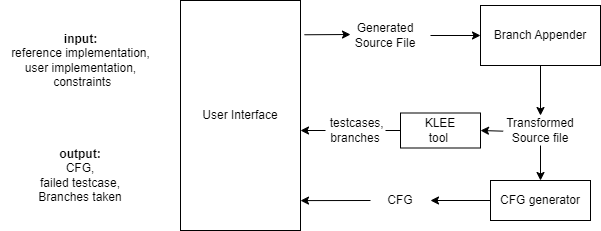
\includegraphics[width=1\textwidth]{3/systemarchi.png}
\caption{Architecture Diagram }
\label{fig:arch}
\end{figure}


\subsection{CONTROL FLOW GRAPH GENERATOR}

Clang is a C/C++/Objective-C compiler front-end. It is a sub-project of LLVM and uses LLVM for code optimization and back-end support. LLVM is a set of compiler and toolchain technologies that can be used to develop a front end for any programming language and a back end for any instruction set architecture. LLVM is designed around a language-independent intermediate representation (IR) that serves as a portable, high-level assembly language that can be optimized with a variety of transformations over multiple passes.Figure \ref{fig:llvm} shows how source code, clang, LLVM IR and LLVM are connected.

\begin{figure}[h]
\centering
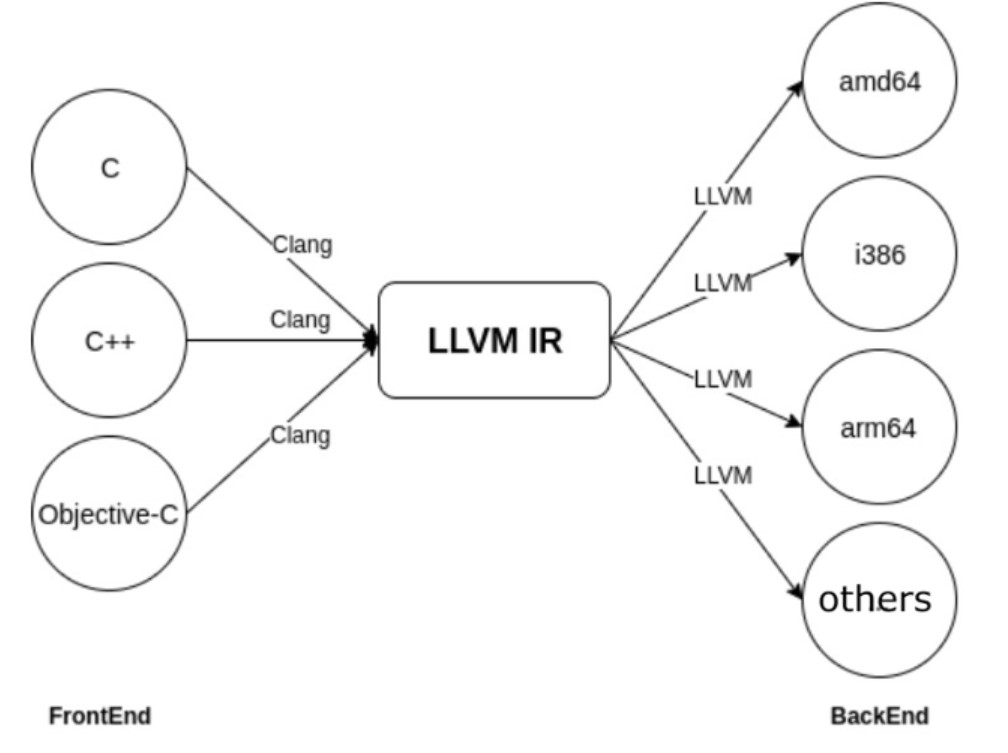
\includegraphics[width=1\textwidth]{3/llvm.jpg}
\caption{Structure of clang/llvm compiler}
\label{fig:llvm}
\end{figure}
Clang provides different interfaces that we can choose from to write a clang-tool. LibTooling is a library to support writing standalone tools based on Clang using which this module is implemented.Constructions of CFG procceds as follows using the above library :  Locating function declarations in the code by identifying nodes representing them in AST(Abstract Syntax Tree) generated by Clang,Accessing AST-Clang holds AST nodes in ASTContext which is defined in ASTContext.h. Clang’s library has prepared an abstract interface, ASTConsumer, which is defined in ASTConsumer.h. We have to define a new object that inherits ASTConsumer,  Reading AST-ASTConsumer has many methods for reading the AST. We are using HandleTranslationUnit (clang::ASTContext&) which is invoked when AST of each translation unit is parsed. This method is empty and we must override it, clang::ast\_matchers::MatchFinder class checks if there is a "matching node" in the context or not, clang::ast\_matchers::MatchFinder:: MatchCallback is a "callback" object which is called when the “matching node” that is registered for it is successfully found in the AST. “Finder” calls this method and passes the information of the “matching node” as an argument with type const \hspace{20} clang::ast\_matchers::MatchFinder::
MatchResult to it, The run function in callback object uses clang::CFG::buildCFG to finally construct the CFG.


\begin{figure}[h]
\centering
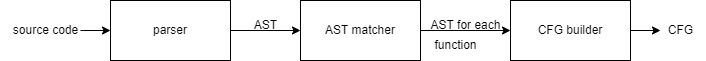
\includegraphics[width=1\textwidth]{3/ast.png}
\caption{Steps for generation of control flow graph (CFG)}
\label{fig:ast}
\end{figure}

\subsection{BRANCH APPENDER}
This Module takes as input the surce file that is generated by the Flask backend and appends print statements that print branch number for corresponding if/else/switch/while/for subblocks.

The source file is parsed by MyFrontEndAction which is a subclass of ASTFrontendAction by overriding  EndSourceFileAction() to create a copy Abstract Syntax Tree(AST) an instance of MYASTConsmer is created which is a subclass of ASTConsumer wherein HandleTopLevelDecl() is overriden to traverse the declarations iteratively and pass them to MyASTVisitor which is a subclass of RecursiveASTVisitor where VisitStmt() is overriden to append siblings in AST - 
 that is to append print branch statements to  if/else/switch/while/for subblocks.

\begin{figure}[h]
\centering
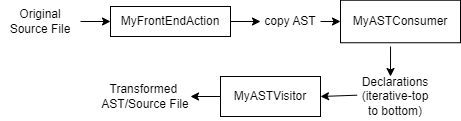
\includegraphics[width=1\textwidth]{3/branchappender.png}
\caption{Branch Appender Module}
\label{fig:graph_compare}
\end{figure}










\subsection{KLEE}
  
A dynamic symbolic execution engine built on top of the LLVM compiler infrastructure is used to automatically generate tests that achieve high coverage on a diverse set of complex and environmentally-intensive program.
  
Dynamic symbolic execution (DSE) is a well-known technique
for automatically generating tests to achieve higher levels of coverage in a program. Two keys ideas of DSE are to seed symbolic execution by executing a program on an initial input and using concrete values from the program execution in place of symbolic expressions whenever symbolic reasoning is hard or not desired.

Its step comprise of Identifying the code under test P and the symbolic inputs to P,Tracing the control flow path p taken by execution reinterpreting program operations to compute symbolic expressions,Generating a path-condition from p and the symbolic expressions,Generating a new input i by negating part of the path-condition, translating the path-condition to the input language of an ATP which stands for automated theorem prover which is a  computer program that show that some statement  is a logical consequence of a set of statements the axioms , invoking the ATP, and lifting a satisfying model back up to the source level,Guiding the search to expose new paths.

 

\begin{figure}[h]
\centering
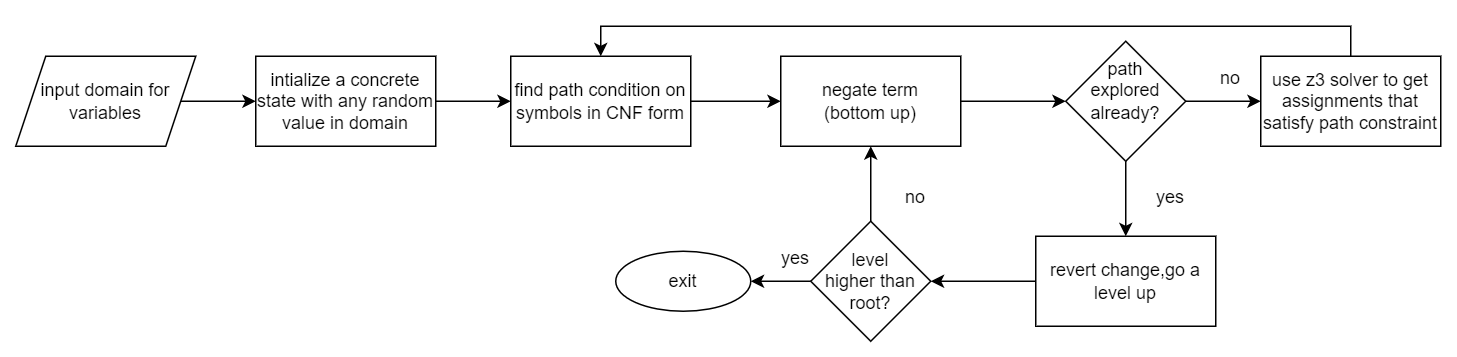
\includegraphics[width=1\textwidth]{3/k.png}
\caption{Dynamic Symbolic Execution procedure}
\label{fig:path}
\end{figure}

\subsection{USER INTERFACE}

The user interface uses jinja2 templates for frontend and flask for backend.The necessary headers,user program,reference program,argument type and constraints are received from the user.The Flask Backend creates new source file and appends these in correct format.shell scripts included in the backend are used to run cfg generator ,branch appender and klee tool  automatically using python's os.system() command .The resultant failed testcase,branches visited in that testcase,and the CFG for both the programs are displayed to the user.
















% Chapter 4

\chapter{\uppercase{Implementation }} % Main chapter title
\label{chap4} % For referencing
This chapter deals with the modules and submodules involved in implementing the Automated Diagnosis of Logical Errors in C programs.
\section{\uppercase{Testcase Generation}}
The testcase for a particular source code is generated using the KLEE tool.To test a function with KLEE, we need to run it on symbolic input. To mark a variable as symbolic, the klee\_make\_symbolic function (defined in klee/klee.h) is used,which takes three arguments: the address of the variable (memory location) that we want to treat as symbolic, its size, and a name for the variable.
\begin{algorithm}
\caption{Marking input as symbolic}\label{alg:cap}
\textbf{Input:} Source Code\\
\textbf{Output:} Total number of instructions, completed paths, partially completed paths and testcases
\begin{algorithmic}[1]
\State Get the variables that is passed in the main function $num$
\State Call klee\_make\_symbolic($num$, sizeof($num$), "num")
\State Return total number of instructions, completed paths, partially completed paths and testcases
\end{algorithmic}
\end{algorithm}
KLEE operates on LLVM bitcode. To run a program with KLEE, the souce code is first compiled into to LLVM bitcode using clang -emit-llvm which is a bitcode file in LLVM bitcode format that is produced using the following command line statement. The -I parameter tells the compiler where to look for klee/klee.h, which defines the intrinsic functions like klee make symbolic that are needed to communicate with the KLEE virtual machine.The bitcode file's debug information is added with the -g option, The bitcode file that was given to KLEE shouldn't be optimised because KLEE has already chosen the appropriate optimisations, which can be activated using the —optimize command-line option.The klee tool is run with the bitcode file for generation of testcases.


\section{\uppercase{Generation of Source Level Control Flow Graph}}
This section discusses the steps involved in generating the control flow graph from the source code in a block format.

The below code does the following steps the source code is taken and a name is assigned through the OptionCategory function.The command line arguments are passed through the OptionsParser.The Clang tool is initialized using the OptionsParser to getSourcePathList() - what files are going to be compiled and getCompilations()- what type of file the source code is to be compiled to.Using Tool.run a new ToolFactory is created.
\begin{algorithm}
\caption{Running the Clang Tool}\label{alg:cap}
\begin{algorithmic}[1]
\State Create CFGCategory as an llvm::cl::OptionCategory
\State Create OptionsParser as a clang::tooling::CommonOptionsParser
\State Create ClangToolTool with OptionsParser's Compilations and SourcePathList
\State Run Tool with ToolFactory
\end{algorithmic}
\end{algorithm}

\newline\newline
FrontendAction is an interface that allows execution of user specific actions as part of the compilation. To run tools over the AST clang it provides a convenient interface called ASTFrontendAction, which takes care of executing the action. 
\begin{algorithm}
\caption{Creating a FrontendAction}\label{alg:cap}
\begin{algorithmic}[1]
\State \textbf{Define} class MyFrontendAction
\State \textbf{Create} member unique pointer of type clang::ASTConsumer
\State \textbf{Implement} function CreateASTConsumer(lang::CompilerInstance\&, llvm::StringRef) to \Return ASTConsumer
\end{algorithmic}
\end{algorithm}

ASTConsumer is an interface used to write generic actions on an AST, regardless of how the AST was produced. ASTConsumer provides many different entry points, HandleTranslationUnit is used here, which is called with the ASTContext for the translation unit.

\begin{algorithm}
\caption{Creating an ASTConsumer}\label{alg:cap}
\begin{algorithmic}[1]
\State class MyConsumer
\State \qquad MyCallback handler;  
\State \qquad clang::ast\_matchers::MatchFinder match\_finder
 \\ \qquad function handler()\\
\qquad\qquad matching\_node = clang::ast\_matchers::functionDecl(clang:: \\ \qquad\qquad ast\_matchers::MainFile()).bind(name)
\\ \qquad function HandleTranslationUnit(clang::ASTContext& ctx)\\
			\qquad\qquad match\_finder.matchAST(ctx);

\end{algorithmic}
\end{algorithm}

\begin{algorithm}
\caption{Print the Graph in Blocks (in class method MyCallback.run)}\label{alg:cap}
\begin{algorithmic}[1]
\State Function $\leftarrow$ Result.Nodes.getNodeAs$<$clang::FunctionDecl$>$()
\State CFG $\leftarrow$ clang::CFG::buildCFG(Function, Function-$>$getBody(), Result.Context, clang::CFG::BuildOptions())
\For{blk in CFG}
   \State blk-$>$dump()
\EndFor
\end{algorithmic}
\end{algorithm}

\section{\uppercase{Boost Graph Generation}}
Boost Graph Library is a generic interface that allows access to a graph's structure, but hides the details of the implementation. This is an “open” interface that is any graph library that implements this interface will be interoperable with the BGL generic algorithms and with other algorithms that also use this interface.The BGL graph interface and graph components are generic, in the same sense as the Standard Template Library (STL). The algorithm \ref{alg:boost-AST} is used to generate a source level graph.
\begin{algorithm}
\caption{Boost Graph Generation from AST}\label{alg:boost-AST}
\begin{algorithmic}[1]
\State Initialize vertex $v$ to zero
\State Create a vector container $E$ for edges
\State Create a vector container $L$ for labels
\State Create a map $M$
\For{$b \in$ CFG}
    \State $x \gets$ Function.getNameAsString() + $b$.getBlockID()
    \If {$M$.find($x$) $==$ $M$.end()}
        \State $M[x] \gets v$
        \State increment $v$
        \State $str \gets$ ""
        \State llvm.raw\_string\_ostream output($str$)
        \For{each block instance $i$}
            \State $i$.dumpToStream(output)
            \If {$b$.getTerminator().isValid()}
                \State $b$.printTerminator(output)
            \EndIf
            \State $L$.push\_back($str$)
        \EndFor
        \For{each successive block instance $i$}
            \State $y \gets$ Function.getNameAsString() + $b$.getBlockID()
            \If {$M$.find($y$) $==$ $M$.end()}
                \State $M[y] \gets v$
                \State increment $v$
                \State $str \gets$ initialize a string
                \State llvm.raw\_string\_ostream output($str$)
                \For{each block instance $i$}
                    \State $i$.dumpToStream(output)
                    \State $L$.push\_back($str$)
                \EndFor
            \EndIf
            \State $E$.push\_back(($M[x]$, $M[y]$))
        \EndFor
    \EndIf
\EndFor
\end{algorithmic}
\end{algorithm}

\section{\uppercase{Error Branch Detection}}
This section focuses on identifying the branches in the program that causes an error - that is wrong branch was taken or a branch was missing altogether for some test case.The test cases are identified that caused the error as well as the corresponding branches that were taken in the reference program as compared to the user program and identify the branch error. 

The Abstract Syntax Tree (AST) generated using Clang can be used to automatically insert statements after control flow statements. This can be achieved by traversing the AST and inserting the desired statement after each control flow statement. 

For instance if a statement is to be inserted after a while loop, the AST can be traversed to find the while loop and then the statement can be inserted as a sibling node of the while loop in the AST. This process can be repeated for other control flow statements, such as if-statements, for-loops and switch-statements.

By using the AST generated using Clang, it is possible to automatically insert statements after control flow statements in a program. This can be a useful tool for labeling all the branches of the program.

The algorithm below explains the steps involved in this process.
\begin{algorithm}
\caption{Error Branch Detection}\label{alg:error-detection}
\begin{algorithmic}[1]
\For{each source file}
    \State Create copy of Abstract Syntax Tree (AST)
    \For{each statement in AST}
        \If{statement type in \{'if-else', 'while', 'for'\}}
            \State Append branch number to body
        \EndIf
    \EndFor
    \State Generate c file with appended branch numbers
    \State Use KLEE to generate testcases and assert return value of user and reference program
    \State Use KLEE to find testcase that fails assertion
    \State Identify corresponding branches in user program that caused the error
\EndFor
\end{algorithmic}
\end{algorithm}
% Chapter 5

\chapter{\uppercase{Results}} % Main chapter title
\label{chap5} % For referencing
To use the program, the user has to first input the headers used. The headers for klee and assert must not be included. The user must also enter the name of the functions (reference and error implementation) and the definition of these functions. The user then has to select the type of argument needed by the functions and any additional constraints on the input.\\
\begin{figure}[h]
\centering
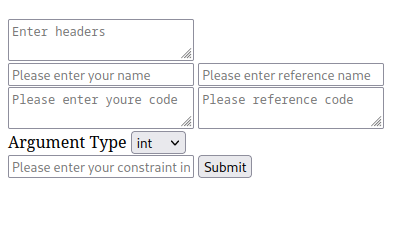
\includegraphics[width=1\textwidth]{5/ui.png}
\caption{User Interface for the program}
\label{fig:ui}
\end{figure}
The program was tested using some programs that are attached in the appendix. These programs were chosen to depict errors that arise from different mistakes in programming. Additional information about these programs are given in the table \ref{tab:my_label}. \\\\

\begin{table}[ ]
    \centering
    \begin{tabularx}{\textwidth} { 
        | >{\raggedright\arraybackslash}X |
        | >{\centering\arraybackslash}X 
        | >{\centering\arraybackslash}X 
        | >{\centering\arraybackslash}X 
        | >{\centering\arraybackslash}X 
        | >{\centering\arraybackslash}X 
        | >{\raggedleft\arraybackslash}X | }
        \hline
        Program & Error Type & LOC (ref) & LOC (err) & Iterative & Recursive & Time \\
        \hline
        isVowel & Incorrect Branch & 34 & 29 & False & False & 1.024  \\
        \hline
        isPrime & Loop Start & 13 & 13 & True & False & 0.903  \\
        \hline
        isPrime & Loop End & 13 & 13 & True & False & 1.089  \\
        \hline
        isPrime & Loop Increment & 13 & 13 & True & False & 0.890  \\
        \hline
        isPrime & Infinite Loop & 13 & 13 & True & False & 46.245  \\
        \hline
        fib & Incorrect Recursion & 10 & 9 & False & True & 0.744  \\
        \hline
    \end{tabularx}
    \caption{Time taken for testing of the C Programs}
    \label{tab:my_label}
\end{table}
The time taken to detect the error was greatest in the case of the infinite loop error type. The other errors were detected in about 1 second when an appropriate constraint was given. The runtime varies depending on various external factors.

The above information is depicted graphically in the chart \ref{fig:runtime}.\\
\begin{figure}[h!]
  \centering
    \begin{tikzpicture}[trim axis left]
        \begin{axis}  
        [  
            scale only axis,
            ybar,  
            width=\textwidth,
            ylabel={\ Time in seconds}, % the ylabel must precede a # symbol.  
            x tick label style = {font = \small, text width = 1.7cm, align = center, rotate = 70, anchor = north east},
            symbolic x coords={Incorrect Branch, Loop Start, Loop End, Loop Increment, Infinite Loop, Incorrect Recursion}, % these are the specification of coordinates on the x-axis.  
            xtick=data,  
             nodes near coords, % this command is used to mention the y-axis points on the top of the particular bar.  
            nodes near coords align={vertical},  
            ]  
        \addplot coordinates {(Incorrect Branch,1.024) (Loop Start,0.903) (Loop End,1.089) (Loop Increment,0.890) (Infinite Loop,46.245) (Incorrect Recursion,0.744) };  
        \end{axis}  
    \end{tikzpicture}
  \caption{C statements vs Time taken for execution}
  \label{fig:runtime}
\end{figure}
%% Chapter 6

\chapter{\uppercase{Comparison}} % Main chapter title
\label{chap6} % For referencing
This chapter is optional. Depending on the work, comparison can also be included in previous chapter.


\chapter{\uppercase{Conclusion and Future Work}}
\label{chap:conclusion}
\section{\uppercase{CONCLUSION}}
This documentation explains the working of automatic diagnosis of logical errors based on a reference implementation and testcases generated for a particular source code.The KLEE tool was implemented for testcase generation and using clang libraries the control flow graph is generated and error localization is performed to mark the lines that have an error.
\section{\uppercase{FUTURE WORK}}
Future works will aim to find a way to enhance the localisation of logical errors and suggest solutions to those errors that were localised in a particular source code.This will help programmers to code easily and save time in fixing these logical errors
\cleardoublepage
\phantomsection 
\appendix
\addcontentsline{toc}{chapter}{APPENDIX}
\chapter{\uppercase{Topic 1}}
\section{Logical Errors in Simple Conditional Statements}
\subsection{Switch Case}
In the following algorithm to determine if a character is vowel user had made a typo by entering j instead of i which leads to wrong outputs for both i and j.
\subsubsection{Reference Implementation for Incorrect Branch }
\begin{verbatim}
int isvowel_r(char n) {
    switch(n) {
        case 'a':
            {
                return 1;
                break;
            }
        case 'e':
            {
                return 1;
                break;
            }
        case 'i':
            {
                return 1;
                break;
            }
        case 'o':
            {
                return 1;
                break;
            }
        case 'u':
            {
                return 1;
                break;
            }
        default:
            {
                return 0;
            }
    }              

}
\end{verbatim}
\subsubsection{Error-ridden Implementation for Incorrect Branch}
\begin{verbatim}
int isvowel_i(char n) {
    switch(n) {
        case 'a': 
            {
                return 1;
            }
        case 'e':
            {
                return 1;
            }
        case 'j': 
            {
                return 1;
            }
        case 'o':
            {
                return 1;
            }
        case 'u':
            {
                return 1;
            }

        default:
            {
                return 0;
            }
    }              
}
\end{verbatim}
\subsubsection{Main Function for Incorrect Branch}
\begin{verbatim}
int main(){
    char n;
    klee_make_symbolic(&n, sizeof(n), "n");
    klee_assume(n>='a' && n<='z');
    assert(isvowel_r(n)==isvowel_i(n));
}
\end{verbatim}
\subsubsection{Branch-Appended Reference Implementation for Incorrect Branch}
\begin{verbatim}
int isvowel_r(char n) {
    switch(n) {
        case 'a':
            {
                printf("in branch 5\n");{
                return 1;
                break;
            }
}
        case 'e':
            {
                printf("in branch 4\n");{
                return 1;
                break;
            }
}
        case 'i':
            {
                printf("in branch 3\n");{
                return 1;
                break;
            }
}
        case 'o':
            {
                printf("in branch 2\n");{
                return 1;
                break;
            }
}
        case 'u':
            {
                printf("in branch 1\n");{
                return 1;
                break;
            }
}
        default:
            {
                printf("in branch 0\n");{
                return 0;
            }
}
    }              

}

\end{verbatim}

\subsubsection{Branch-Appended Error-ridden Implementation for Incorrect Branch}
\begin{verbatim}
int isvowel_i(char n) {
    switch(n) {
        case 'a': 
            {
                printf("in branch 11\n");{
                return 1;
            }
}
        case 'e':
            {
                printf("in branch 10\n");{
                return 1;
            }
}
        case 'j': 
            {
                printf("in branch 9\n");{
                return 1;
            }
}
        case 'o':
            {
                printf("in branch 8\n");{
                return 1;
            }
}
        case 'u':
            {
                printf("in branch 7\n");{
                return 1;
            }
}

        default:
            {
                printf("in branch 6\n");{
                return 0;
            }
}
    }              
}
\end{verbatim}
\subsubsection{Result for Incorrect Branch}
\textbf{Input Information}
\begin{verbatim}
object 0: name: 'n'
object 0: size: 1
object 0: data: b'j'
object 0: hex : 0x6a
object 0: int : 106
object 0: uint: 106
object 0: text: j
\end{verbatim}
\textbf{Branches Accessed}
\begin{verbatim}
in branch 0
in branch 9
\end{verbatim}
\begin{figure}[h]
\centering
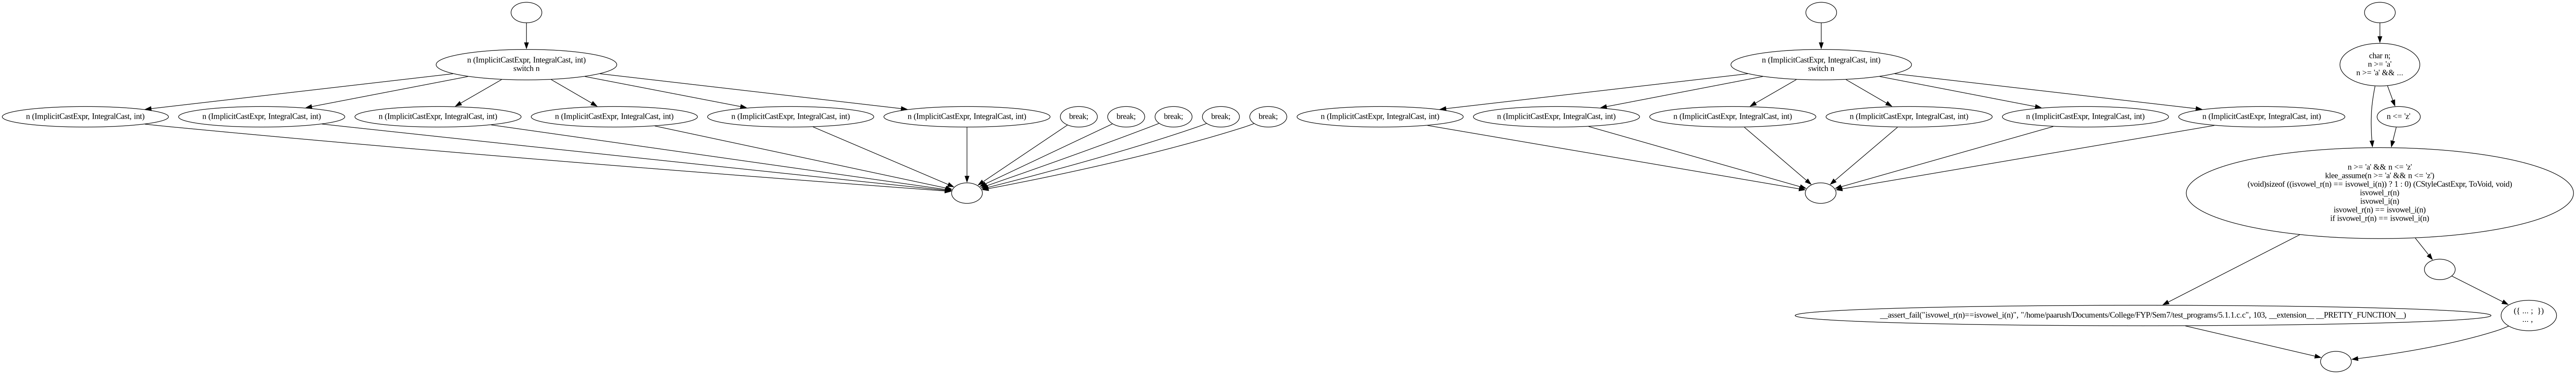
\includegraphics[width=1\textwidth]{5/5.1.1.c.png}
\caption{CFG for Program 5.1.1}
\label{fig:cfg5.1.1}
\end{figure}
\subsubsection{Result Interpretation for Incorrect Branch}
for test case 'j' the switch case takes action corresponding to default case in reference implementation however not so in user implementation hence the user implementation must have falsely classfied as non-default that is vowel case


\section{Logical Errors in Iteration}
For the following examples we take algorithm to determine if a number is prime and introduce logical errors to them as follows and diagonize them.
\subsection{Intialization error}
Here i is intialized from 1 instead of 2 also corner case isn't handled.
\subsubsection{Reference Implementation for Loop Start Error}
\begin{verbatim}
int isPrime_r(int n)
{
    // Corner case
    if (n <= 1)
        return 0;
    // Check from 2 to square root of n
    for (int i = 2; i <= n-1; i++)
        if (n % i == 0)
            return 0;
    return 1;
}
\end{verbatim}
\subsubsection{Error-ridden Implementation for Loop Start Error}
\begin{verbatim}
int isPrime_i(int n)
{
    if (n <= 1)
        return 0;
    // Check from 2 to square root of n
    for (int i = 1; i <= n-1; i++)
        if (n % i == 0)
            return 0;
    return 1;
}
\end{verbatim}
\subsubsection{Main Function for Loop Start Error}
\begin{verbatim}
int main(){
    int n;
    klee_make_symbolic(&n, sizeof(n), "n");
    klee_assume(n>=0 && n<=10);
    assert(isPrime_r(n)==isPrime_i(n));
}
\end{verbatim}
\subsubsection{Branch-Appended Reference Implementation for Loop Start Error}

\begin{verbatim}
int isPrime_r(int n)
{
    // Corner case
    if (n <= 1)
        {
            printf("in branch 0\n");return 0;}

    // Check from 2 to square root of n
    for (int i = 2; i <= n-1; i++)
        {
            printf("in branch 1\n");if (n % i == 0)
            {
                printf("in branch 2\n");return 0;}}

    return 1;
}
\end{verbatim}

\subsubsection{Branch-Appended Error-ridden Implementation for Loop Start Error}

\begin{verbatim}
int isPrime_i(int n)
{
    // Corner case
    if (n <= 1)
        {
            printf("in branch 3\n");return 0;}

    // Check from 2 to square root of n
    for (int i = 1; i <= n-1; i++)
        {
            printf("in branch 4\n");if (n % i == 0)
            {
                printf("in branch 5\n");return 0;}}
    return 1;
}
\end{verbatim}
\subsubsection{Result for Loop Start Error}
\textbf{Input Information}
\begin{verbatim}
object 0: name: 'n'
object 0: size: 4
object 0: data: b'\x02\x00\x00\x00'
object 0: hex : 0x02000000
object 0: int : 2
object 0: uint: 2
object 0: text: ....
\end{verbatim}


\textbf{Branches Accessed}
\begin{verbatim}
in branch 4
in branch 5
\end{verbatim}
\begin{figure}[h]
\centering
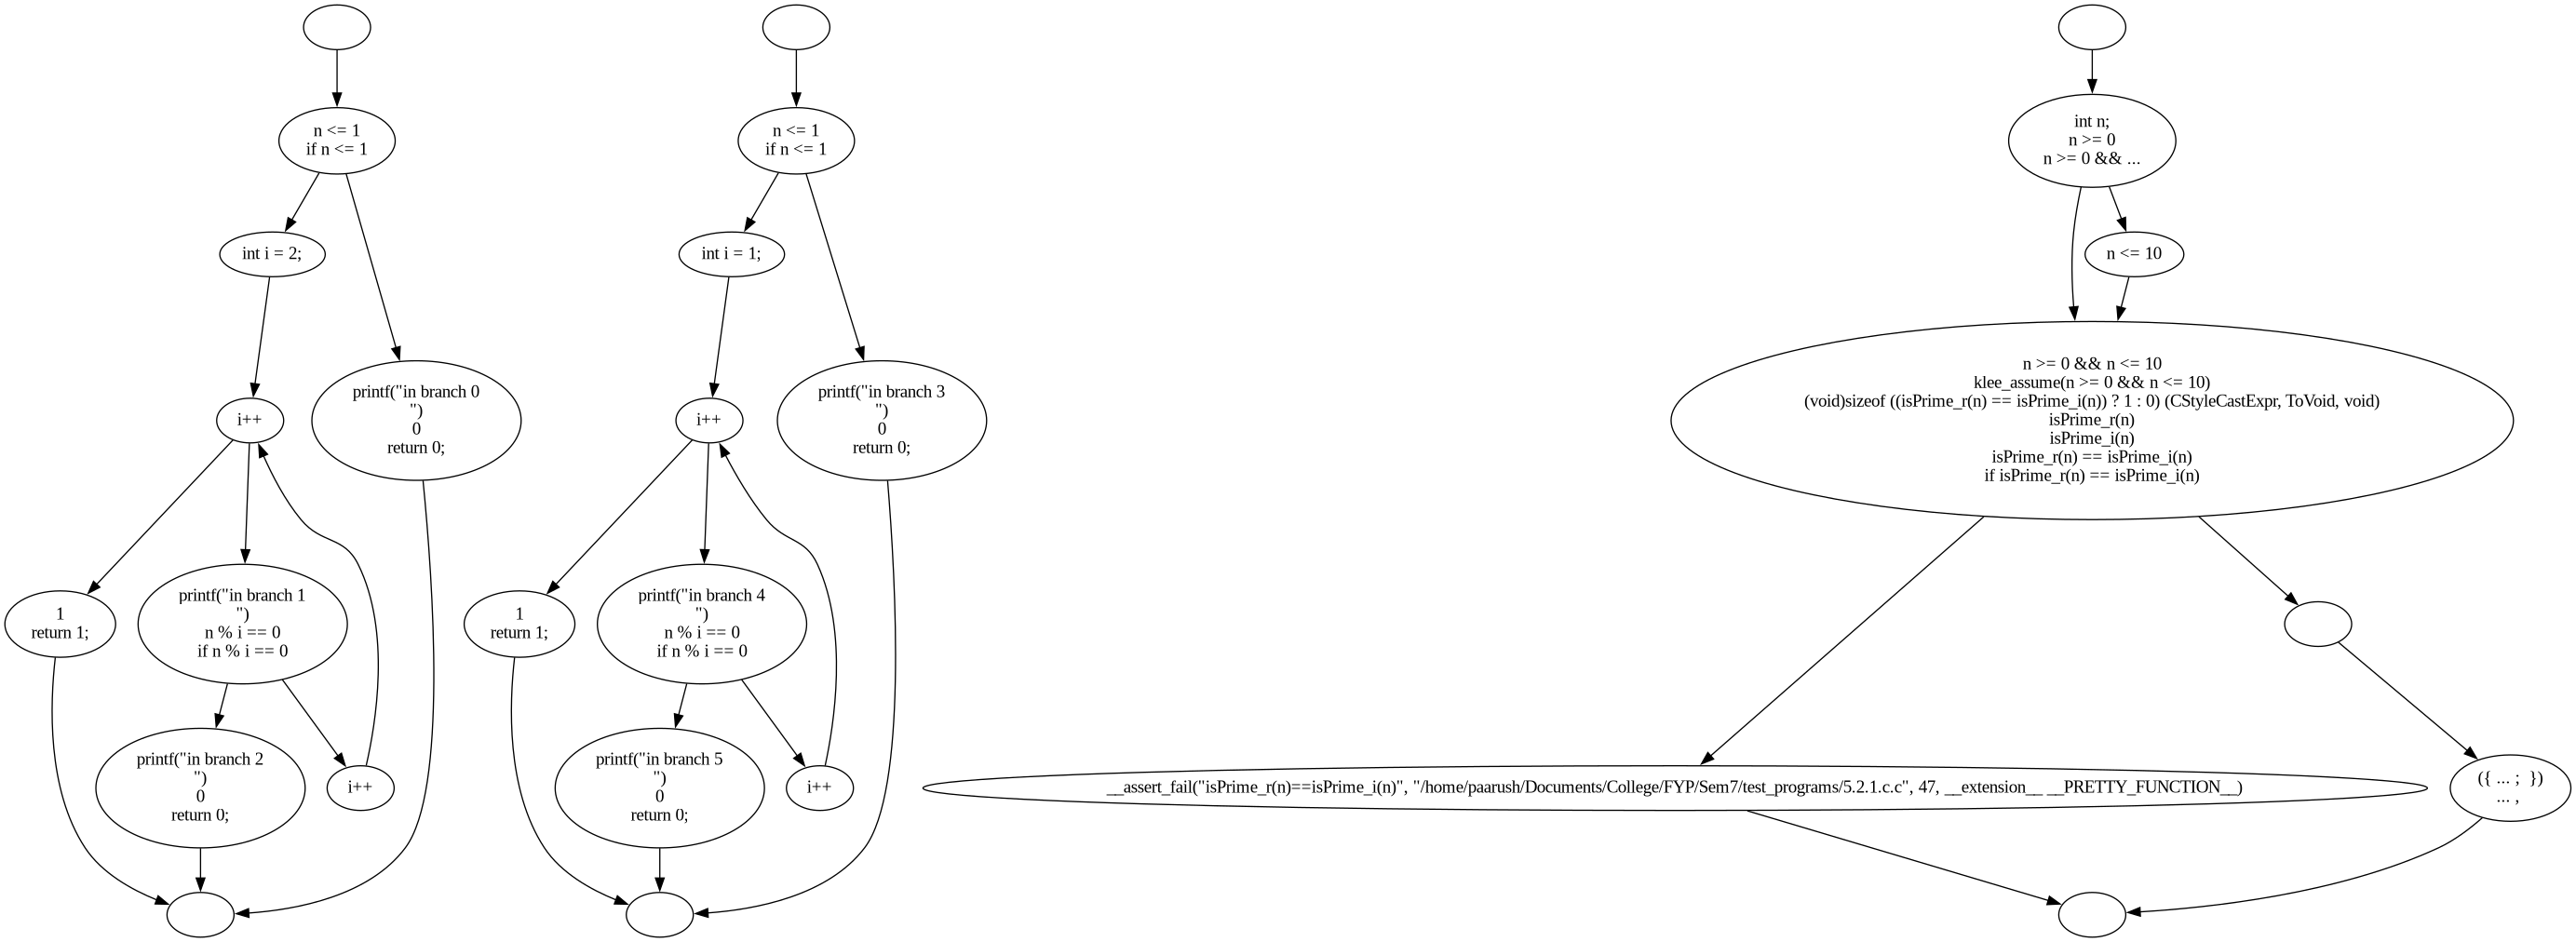
\includegraphics[width=1\textwidth]{5/5.2.1.c.png}
\caption{CFG for Program 5.2.1}
\label{fig:cfg5.2.1}
\end{figure}
\subsubsection{Result Interpretation for Loop Start Error}
for test case value 2 the user implementation had entered branch 4 but reference implementation had not entered branch 2 hence it can be attributed to entry condition error.
\subsection{Termination error}
Here termination is supposed to be $i<=n-1$ however we terminate at $i<=n$
\subsubsection{Reference Implementation for Loop End Error}
\begin{verbatim}
int isPrime_r(int n)
{
    // Corner case
    if (n <= 1)
        return false;
 
    // Check from 2 to square root of n
    for (int i = 2; i <= n-1; i++)
        if (n % i == 0)
            return false;
 
    return true;
}
\end{verbatim}
\subsubsection{Error-ridden Implementation for Loop End Error}
\begin{verbatim}
int isPrime_i(int n)
{
    // Check from 2 to square root of n
    if (n <= 1)
		return 0;
    for (int i = 2; i <= n; i++)
        if (n % i == 0)
            return false;
    return true;
}
\end{verbatim}
\subsubsection{Main Function for Loop End Error}
\begin{verbatim}
int main(){
    int n;
    klee_make_symbolic(&n, sizeof(n), "n");
    klee_assume(n>=0 && n<=10);
    assert(isPrime_r(n)==isPrime_i(n));
}
\end{verbatim}
\subsubsection{Branch-Appended Reference Implementation for Loop End Error}
\begin{verbatim}
int isPrime_r(int n)
{
    // Corner case
    if (n <= 1)
        {
            printf("in branch 0\n");return 0;}

    // Check from 2 to square root of n
    for (int i = 2; i <= n-1; i++)
        {
            printf("in branch 1\n");if (n % i == 0)
            {
                printf("in branch 2\n");return 0;}}

    return 1;
}
\end{verbatim}

\subsubsection{Branch-Appended Error-ridden Implementation for Loop End Error}

\begin{verbatim}
int isPrime_i(int n)
{
    // Corner case
    if (n <= 1)
        {
            printf("in branch 3\n");return 0;}

    // Check from 2 to square root of n
    for (int i = 2; i <= n; i++)
        {
            printf("in branch 4\n");if (n % i == 0)
            {
                printf("in branch 5\n");return 0;}}
    return 1;
}
\end{verbatim}
\subsubsection{Result for Loop End Error}
\textbf{Input Information}
\begin{verbatim}
object 0: name: 'n'
object 0: size: 4
object 0: data: b'\x02\x00\x00\x00'
object 0: hex : 0x02000000
object 0: int : 2
object 0: uint: 2
object 0: text: ....
\end{verbatim}
\textbf{Branches Accessed}
\begin{verbatim}
in branch 4
in branch 5
\end{verbatim}
\begin{figure}[h]
\centering
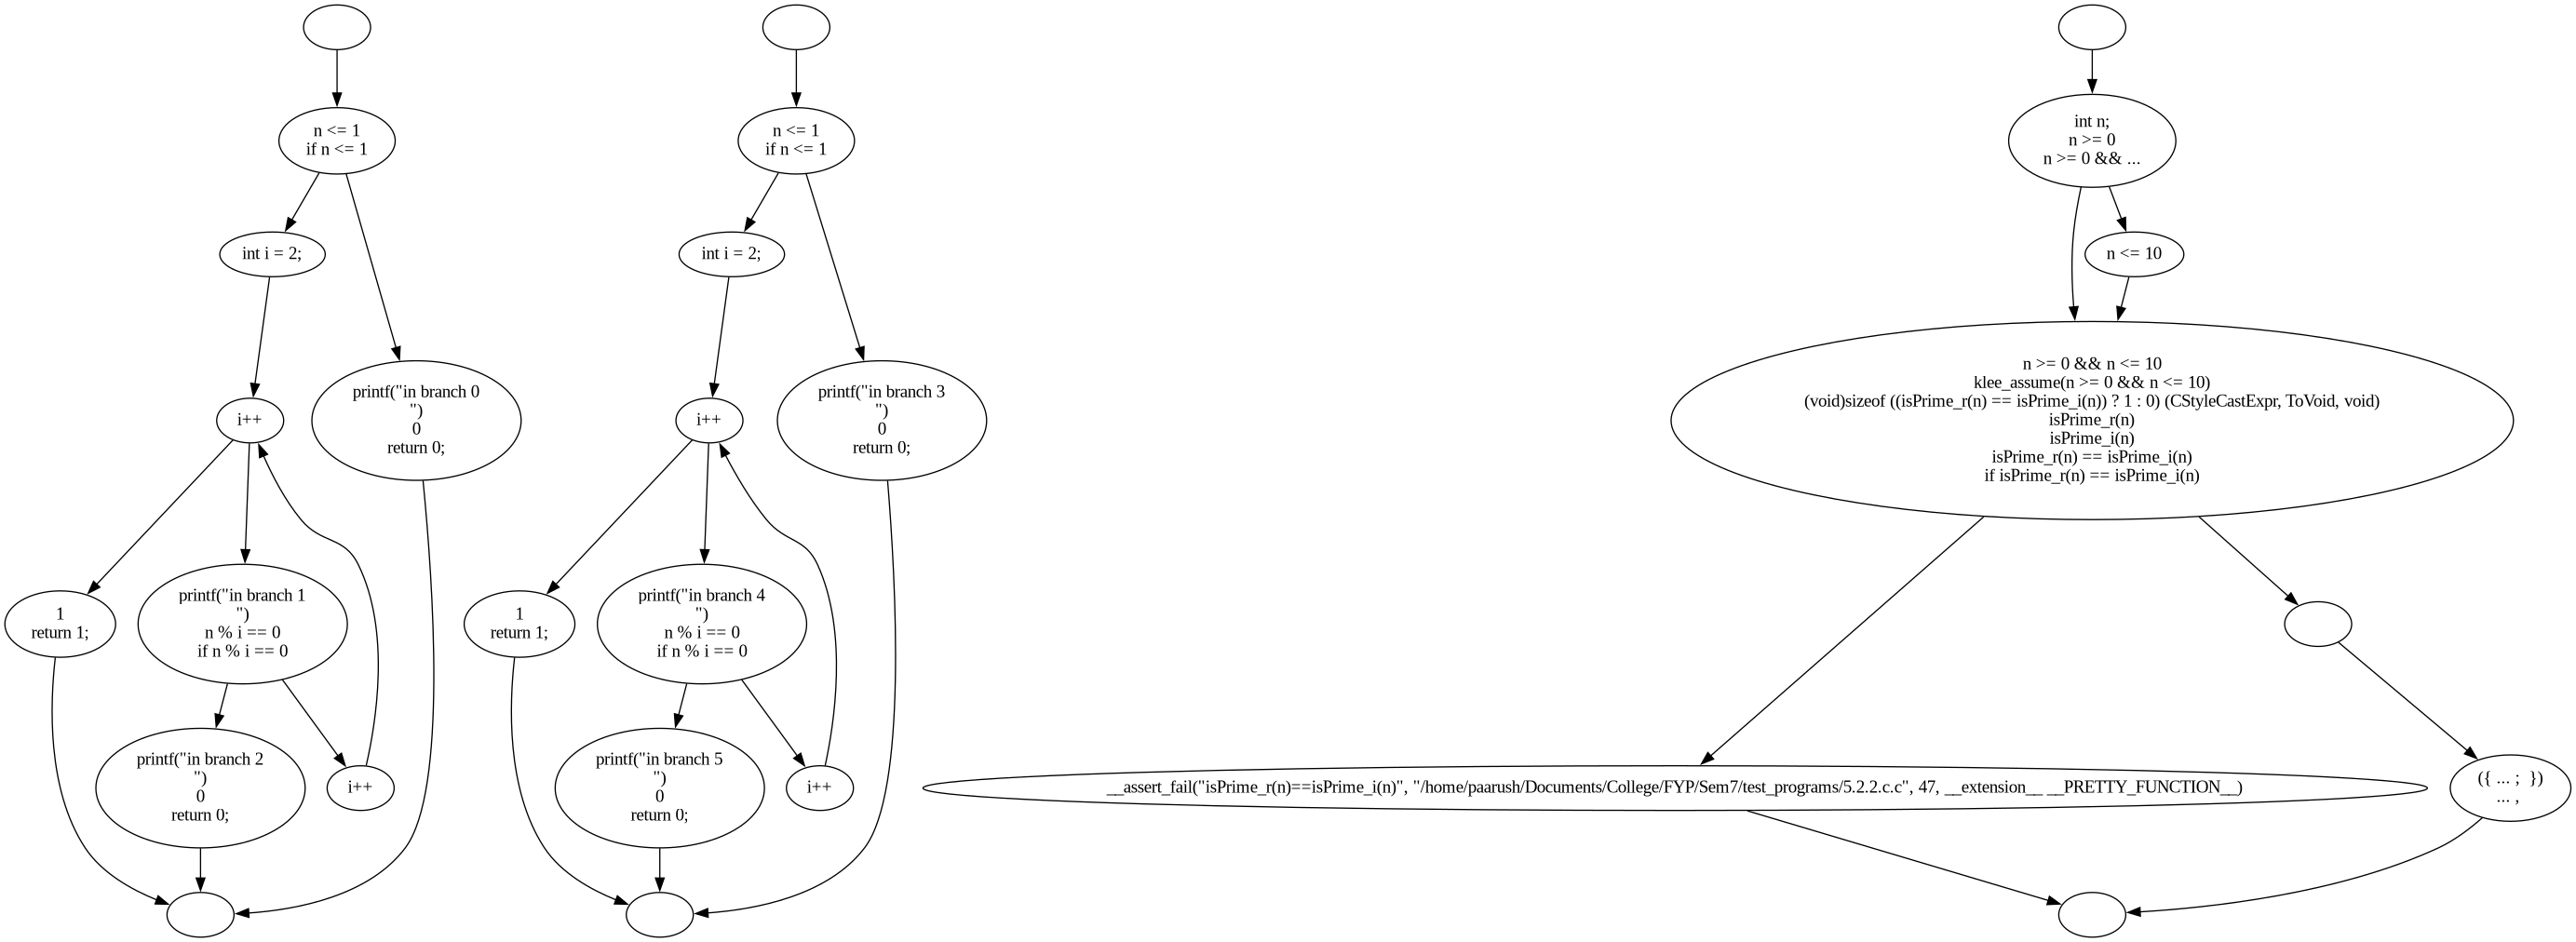
\includegraphics[width=1\textwidth]{5/5.2.2.c.png}
\caption{CFG for Program 5.2.2}
\label{fig:cfg5.2.2}
\end{figure}
\subsubsection{Result Interpretation for Loop End Error}
Here wrong termination condition has failed test case- 2 as 2 enters into branch 4 so it must have staisfied termination constraint hence error can be attributed to it.



\subsection{Control variable updation error}
Here control variable is updated as i+=2 instead of i+=1
\subsubsection{Reference Implementation for Loop Increment Error}
\begin{verbatim}
bool isPrime_r(int n)
{
    // Corner case
    if (n <= 1)
        return false;
 
    // Check from 2 to square root of n
    for (int i = 2; i <= n-1; i++)
        if (n % i == 0)
            return false;
 
    return true;
}
\end{verbatim}
\subsubsection{Error-ridden Implementation for Loop Increment Error}
\begin{verbatim}
bool isPrime_i(int n)
{
    // Corner case
      if (n <= 1)
        return false;
 
    // Check from 2 to square root of n
    for (int i = 2; i <= n-1;i+=2 )
        if (n % i == 0)
            return false;
 
    return true;
}
\end{verbatim}
\subsubsection{Main Function for Loop Increment Error}
\begin{verbatim}
int main(){
    int n;
    klee_make_symbolic(&n, sizeof(n), "n");
    klee_assume(n>=0 && n<=10);
    assert(isPrime_r(n)==isPrime_i(n));
}
\end{verbatim}
\subsubsection{Branch-Appended Reference Implementation for Loop Increment Error}
\begin{verbatim}
int isPrime_r(int n)
{
    // Corner case
    if (n <= 1)
        {
            printf("in branch 0\n");return 0;}

    // Check from 2 to square root of n
    for (int i = 2; i <= n-1; i++)
        {
            printf("in branch 1\n");if (n % i == 0)
            {
                printf("in branch 2\n");return 0;}}

    return 1;
}
\end{verbatim}

\subsubsection{Branch-Appended Error-ridden Implementation for Loop Increment Error}

\begin{verbatim}
int isPrime_i(int n)
{
    // Corner case
    if (n <= 1)
        {
            printf("in branch 3\n");return 0;}

    // Check from 2 to square root of n
    for (int i = 2; i <= n-1; i+=2)
        {
            printf("in branch 4\n");if (n % i == 0)
            {
                printf("in branch 5\n");return 0;}}

    return 1;
}
\end{verbatim}
\subsubsection{Result for Loop Increment Error}
\textbf{Input Information}
\begin{verbatim}
object 0: name: 'n'
object 0: size: 4
object 0: data: b'\t\x00\x00\x00'
object 0: hex : 0x09000000
object 0: int : 9
object 0: uint: 9
object 0: text: ....
\end{verbatim}
\textbf{Branches Accessed}
\begin{verbatim}
in branch 1
in branch 1
in branch 2
in branch 4
in branch 4
in branch 4
in branch 4
\end{verbatim}
\begin{figure}[h]
\centering
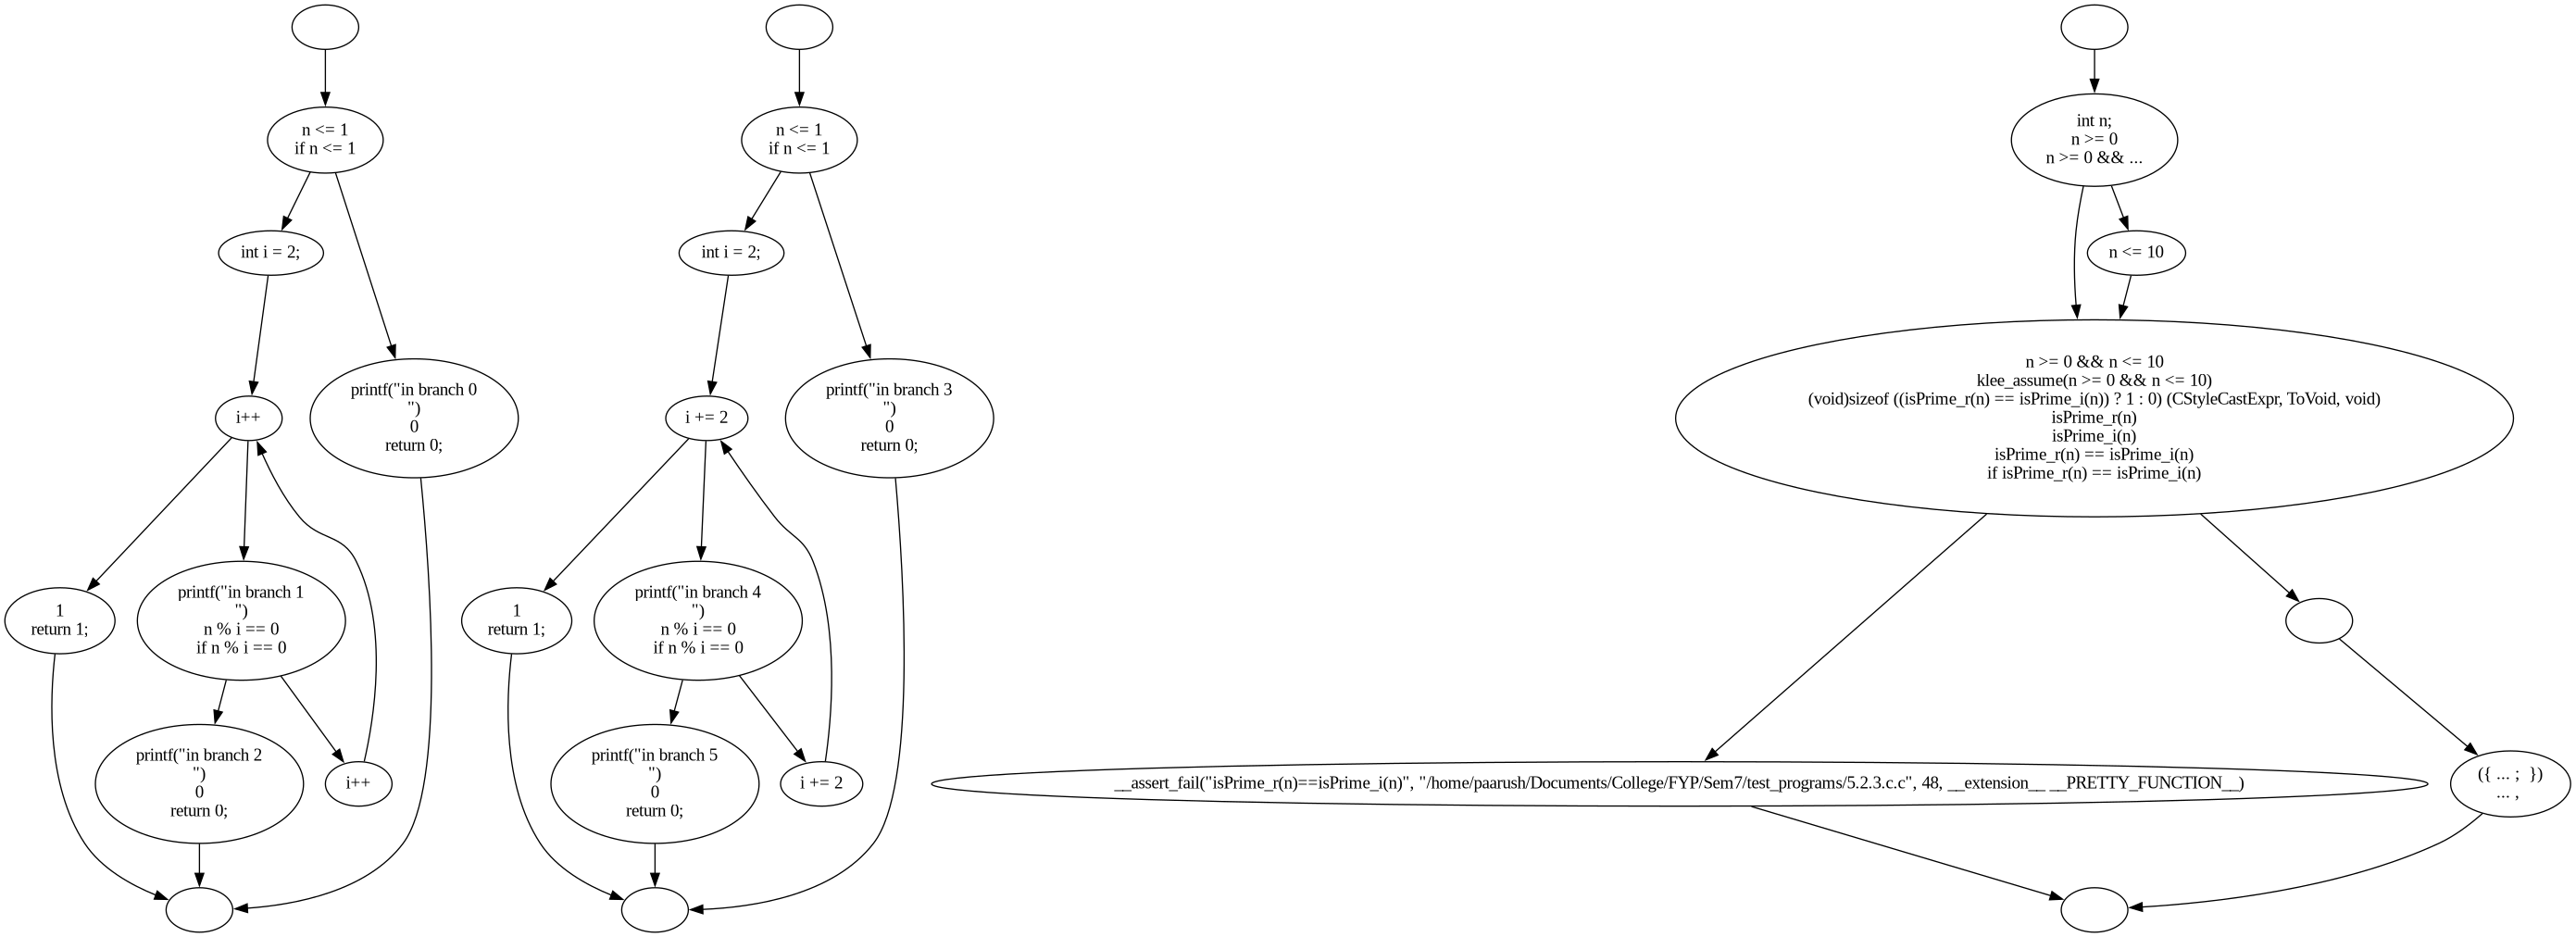
\includegraphics[width=1\textwidth]{5/5.2.3.c.png}
\caption{CFG for Program 5.2.3}
\label{fig:cfg5.2.3}
\end{figure}
\subsubsection{Result Interpretation for Loop Increment Error}
The loop in the reference implementation has run 2 times and on the second run, it has entered branch 2.
The loop in the error implementation has run 4 times and not entered branch 5. This suggests that the loop has completed without reaching the factor. This would mean the factor was skipped and likely is an issue with the increment operator in the for loop.

\subsection{Infinite Loop}
Here incorrect/negligence of termination statement leads to infinite loop
\subsubsection{Reference Implementation for Infinite Loop Error}
\begin{verbatim}
int isPrime_r(int n)
{
    // Corner case
    if (n <= 1)
        return 0;

    // Check from 2 to square root of n
    for (int i = 2; i <= n-1; i++)
        if (n % i == 0)
            return 0;

    return 1;
}
\end{verbatim}
\subsubsection{Error-ridden Implementation for Infinite Loop Error}
\begin{verbatim}
int isPrime_i(int n)
{
    // Corner case
    if (n <= 1)
        return 0;

    // Check from 2 to square root of n
    for (int i = 2; i <= n-1;)
        if (n % i == 0)
            return 0;

    return 1;
}

\end{verbatim}

\subsubsection{Main Function for Infinite Loop Error}
\begin{verbatim}
int main(){
    int n;
    klee_make_symbolic(&n, sizeof(n), "n");
    klee_assume(n>=0 && n<=10);
    assert(isPrime_r(n)==isPrime_i(n));
}
\end{verbatim}
\subsubsection{Branch-Appended Reference Implementation for Infinite Loop Error}
\begin{verbatim}
int isPrime_r(int n)
{
    // Corner case
    if (n <= 1)
        {
            printf("in branch 0\n");return 0;}

    // Check from 2 to square root of n
    for (int i = 2; i <= n-1; i++)
        {
            printf("in branch 1\n");if (n % i == 0)
            {
                printf("in branch 2\n");return 0;}}

    return 1;
}
\end{verbatim}

\subsubsection{Branch-Appended Error-ridden Implementation for Infinite Loop Error}

\begin{verbatim}
int isPrime_i(int n)
{
    // Corner case
    if (n <= 1)
        {
            printf("in branch 3\n");return 0;}

    // Check from 2 to square root of n
    for (int i = 2; i <= n-1; )
        {
            printf("in branch 4\n");if (n % i == 0)
            {
                printf("in branch 5\n");return 0;}}

    return 1;
}
\end{verbatim}
\subsubsection{Result for Infinite Loop Error}
\textbf{Input Information}
\begin{verbatim}
object 0: name: 'n'
object 0: size: 4
object 0: data: b'\t\x00\x00\x00'
object 0: hex : 0x09000000
object 0: int : 9
object 0: uint: 9
object 0: text: ....
\end{verbatim}
\textbf{Branches Accessed}
\begin{verbatim}
in branch 1
in branch 1
in branch 2
in branch 4
in branch 4
in branch 4
in branch 4
...
\end{verbatim}
\begin{figure}[h]
\centering
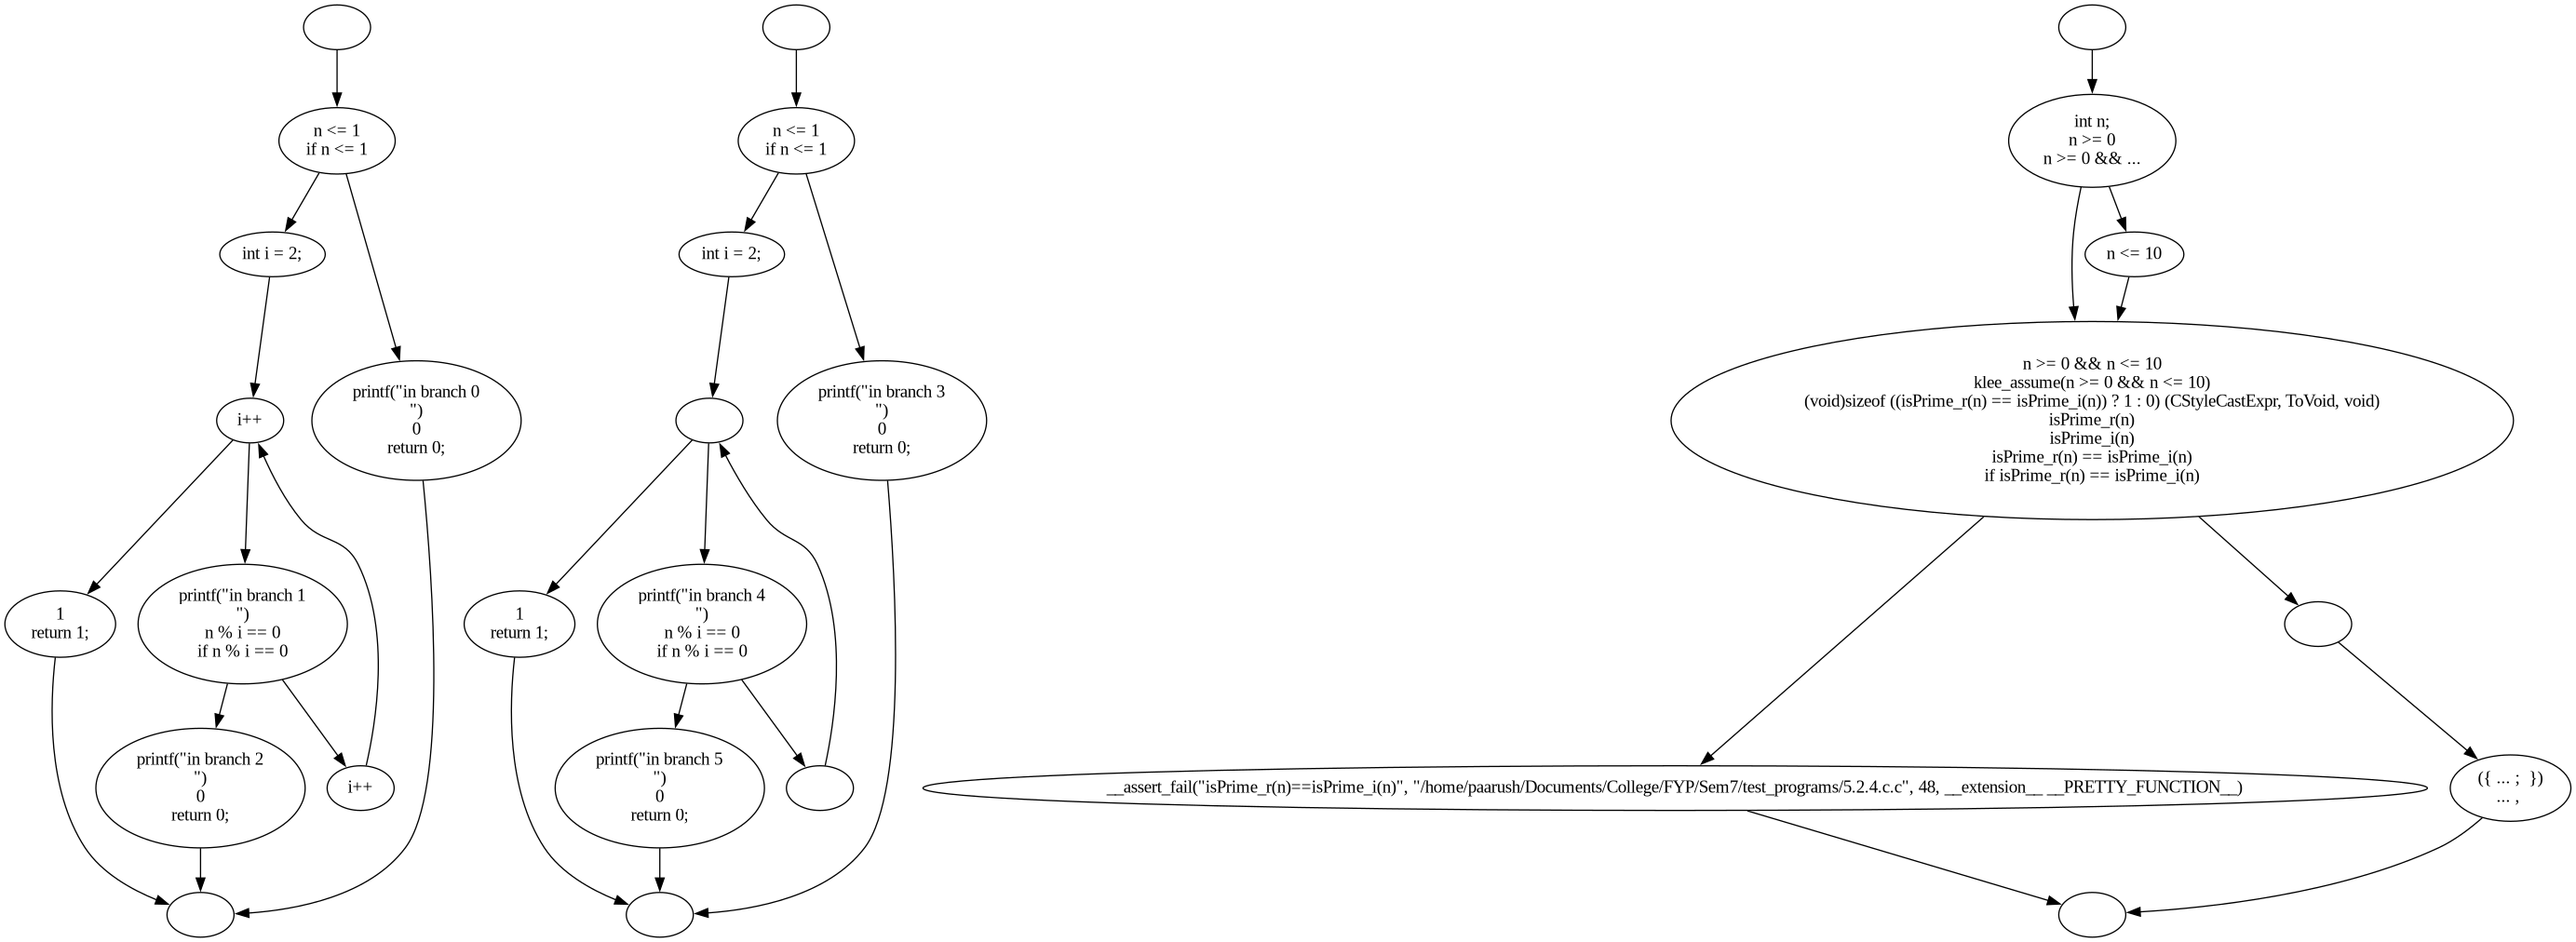
\includegraphics[width=1\textwidth]{5/5.2.4.c.png}
\caption{CFG for Program 5.2.4}
\label{fig:cfg5.2.4}
\end{figure}
\subsubsection{Result Interpretation for Infinite Loop Error}
Here we can notice branch 4 repeatedly visited hence there must be infinite loop in the code.


\section{Logical Errors in Recursion}
\subsection{Errors in Recurrence Relation for Incorrect Recursion Error}
Here error is made in recurrence relation 
$f(x)=f(x-2)+f(x-2)$ instead of $f(x)=f(x-1)+f(x-2)$.
\subsubsection{Reference Implementation for Incorrect Recursion Error}
\begin{verbatim}
int fib_r(int x){
    if (x==0) {
        return 0;
    } else if(x==1){
        return 1;
    }
    else {
        return fib_r(x-2)+fib_r(x-2);
    }
}
\end{verbatim}
\subsubsection{Error-ridden Implementation for Incorrect Recursion Error}
\begin{verbatim}
int fib_i(int x){
    if(x==0) {
        return 0;
    } else if(x==1) {
        return 1;
    } else {
        return fib_i(x-1)+fib_i(x-2);
    }
}
\end{verbatim}
\subsubsection{Main Function for Incorrect Recursion Error}
\begin{verbatim}
int main(){
    int x;
    klee_make_symbolic(&x, sizeof(x), "x");
    klee_assume(x>=0 && x<=5);
    assert(fib_i(x)==fib_r(x));
}
\end{verbatim}
\subsubsection{Branch-Appended Error-ridden Implementation for Incorrect Recursion Error}
\begin{verbatim}
int fib_r(int x){
    if (x==0) {
        printf("in branch 0\n");{
        return 0;
    } }else {
        printf("in branch 1\n");if(x==1){
        printf("in branch 2\n");{
        return 1;
    }
} else {
        printf("in branch 3\n");{
        return fib_r(x-2)+fib_r(x-2);
    }
}}}
\end{verbatim}

\subsubsection{Branch-Appended Reference Implementation for Incorrect Recursion Error}

\begin{verbatim}
int fib_i(int x){
    if(x==0) {
        printf("in branch 4\n");{
        return 0;
    } }else {
        printf("in branch 5\n");if(x==1) {
        printf("in branch 6\n");{
        return 1;
    } }else {
        printf("in branch 7\n");{
        return fib_i(x-1)+fib_i(x-2);
    }
}}}
\end{verbatim}

\subsubsection{Result for Incorrect Recursion Error}
\textbf{Input Information}
\begin{verbatim}
object 0: name: 'x'
object 0: size: 4
object 0: data: b'\x02\x00\x00\x00'
object 0: hex : 0x02000000
object 0: int : 2
object 0: uint: 2
object 0: text: .... 
\end{verbatim}
\textbf{Branches Accessed}
\begin{verbatim}
in branch 5
in branch 7
in branch 5
in branch 6
in branch 4
in branch 1
in branch 3
in branch 0
in branch 0
\end{verbatim}
\begin{figure}[h]
\centering
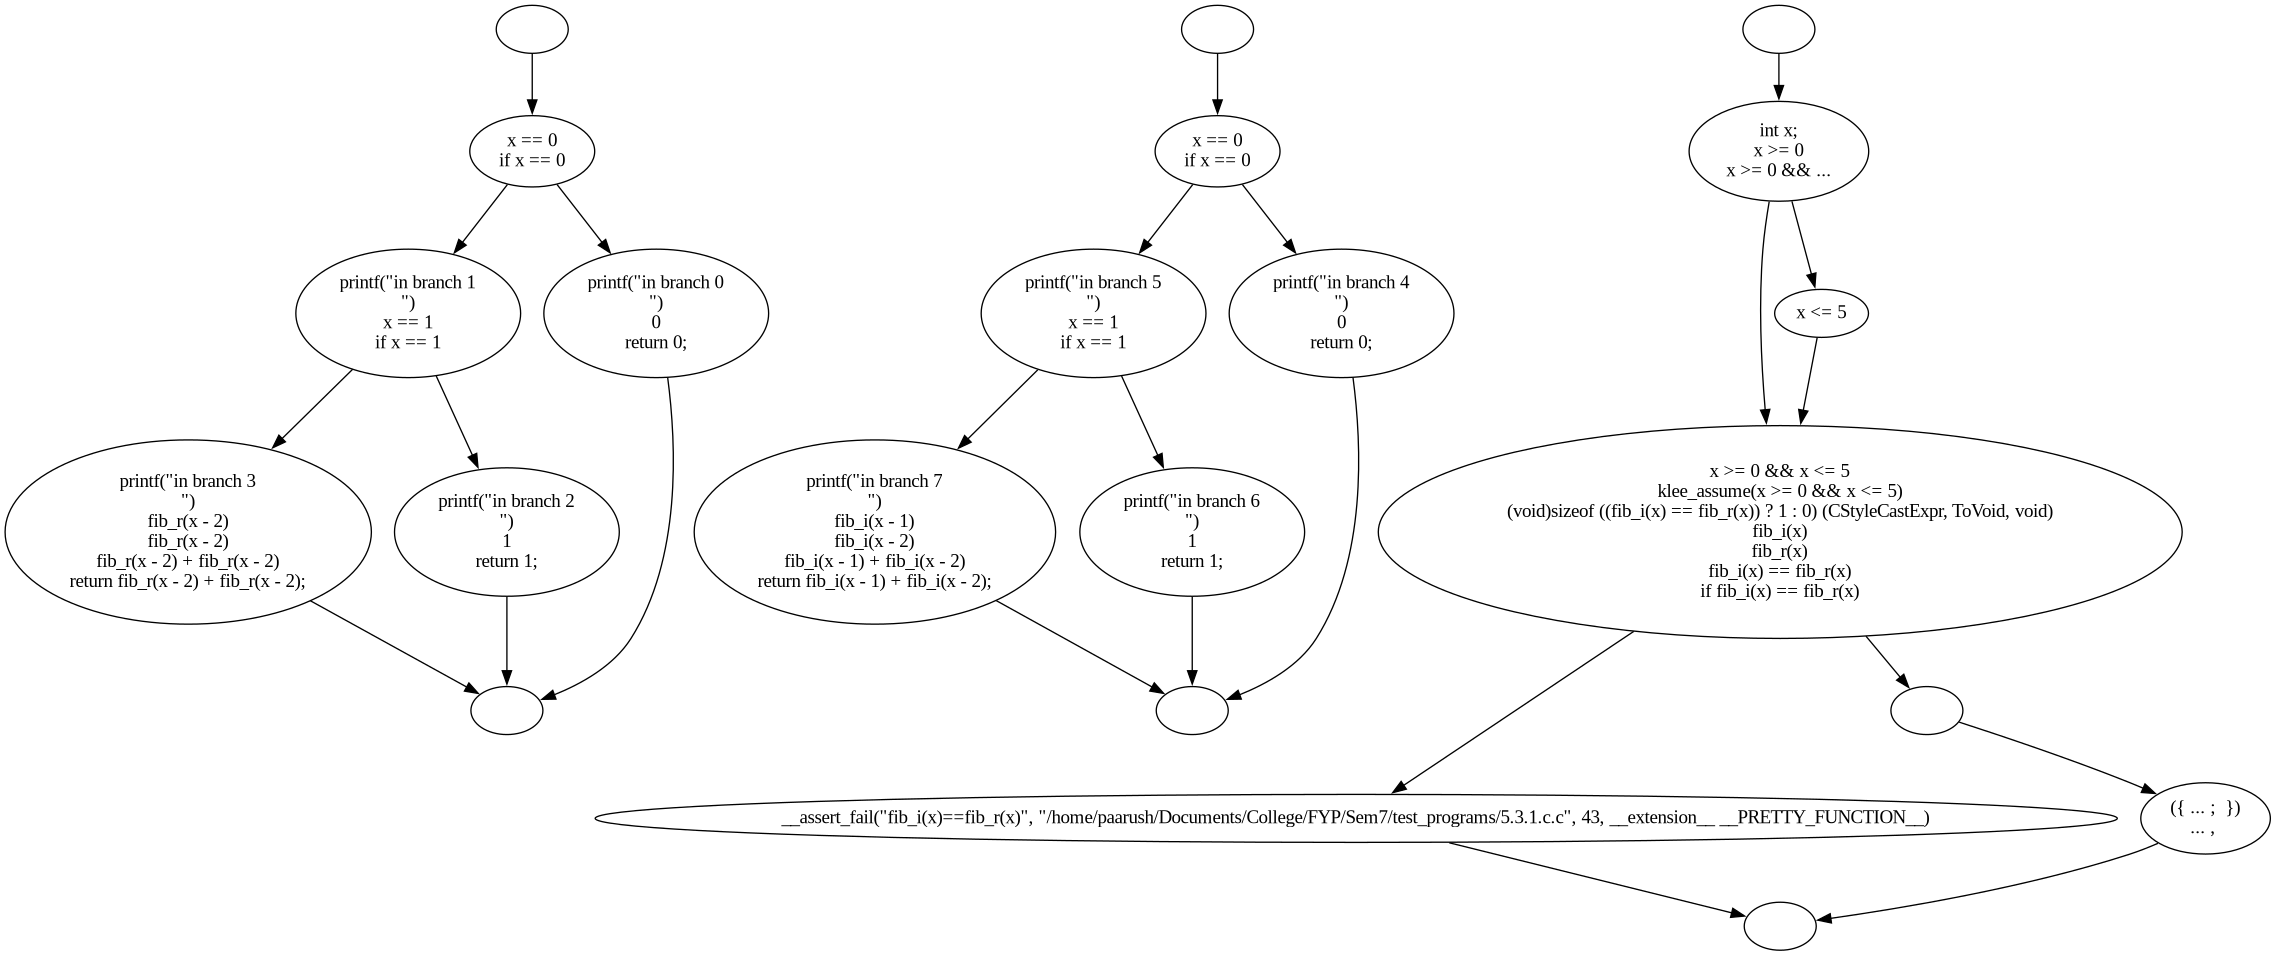
\includegraphics[width=1\textwidth]{5/5.3.1.c.png}
\caption{CFG for Program 5.3.1}
\label{fig:cfg5.3.1}
\end{figure}
\subsubsection{Result Interpretation for Incorrect Recursion Error}
Looking at the similarity in structure of branches correspondence 3-7,1-5,2-6,0-4 can be established  where 0 to 3 belong to user and 4 to 7 belong to reference implementation.
by analyzing patter 5,7,5,6,4 becomes 1,3,1,2,0 which is very different from 1,3,0,0 hence the entire recurrence relation could be attributed to cause of error furthermore 0,0 reflects same branch taken which isn't an expected behaviour from the program







%\bibliographystyle{auapalike}
\bibliographystyle{unsrt}
\nocite{*}%This gives a list of all references that includes without citation. Remove this, once the reference is cited
\phantomsection
\addcontentsline{toc}{chapter}{REFERENCES}
\begin{spacing}{1}
\bibliography{publication}
\end{spacing}

\newpage
\clearpage




\addtocontents{toc}{\protect\newpage}
\addtocontents{lot}{\protect\newpage}
\addtocontents{lof}{\protect\newpage}

\end{document}
